\section{Fit Strategy and Validation}
\label{sec:fit_strategy}
\subsection{SVJ Fit Strategy}
\label{subsec:fit_exclusion}


%Results: An overview of the final fit setup including the final discriminating variables(s), the (SR/CR) regions to be included in the fit and the floating normalization parameters. 
%Some rough first expected limits/discovery sensitivity plots are useful if you have them but not necessary. In this case the binning of the final variable(s) and the systematics smoothing/pruning should be indicated.


%------------------------------------------------- 
\subsubsection{Background Only Fits}
\label{subsec:fit_bkgonly}

Three validations are used for the background fit polynomial: MC across all analysis regions, data in the CR and VR, and pseudo-data in the CR and VR. 

Figure~\ref{fig:postfit_param_pfn} shows the post-fit values of the fit parameters and their uncertainties for the exclusion (PFN-based) CR and VR. 
\begin{figure}[!htbp]
\centering
   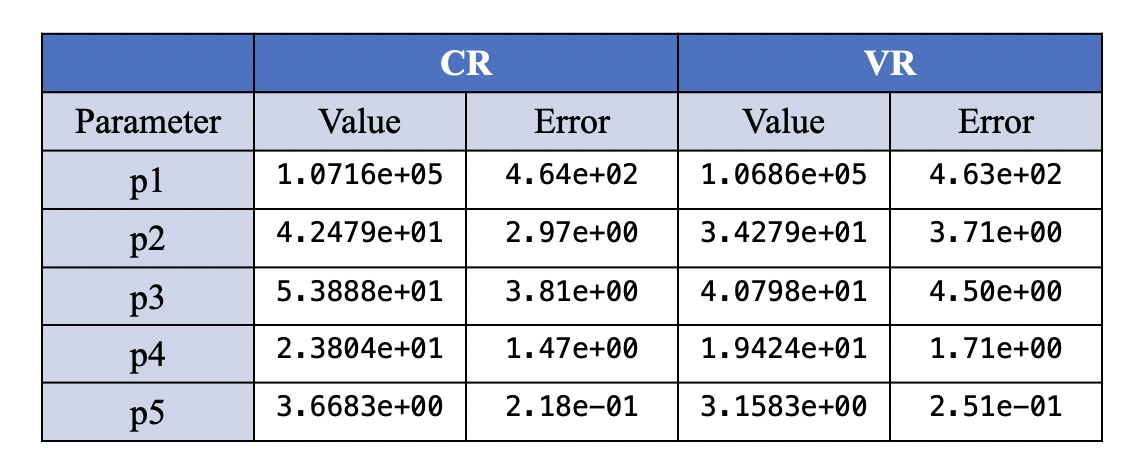
\includegraphics[width=0.65\textwidth]{figures/stats/postfit_param_pfn}
    \caption{Post-fit parameters for the PFN CR and VR.
    \label{fig:postfit_param_pfn}}
\end{figure}

Figure~\ref{fig:bkgfit_mc} shows the ability of this polynomial to fit the smoothly falling \mt~background in simulation across all 3 analysis regions (CR, VR, SR).
The \mt~spectrum is fit in 90 even bins.
These distributions are obtained by downsampling the MC statistics to match the relevant statistics of the data region, in accordance with the MC weights.
The high background-only $p$-value indicates a good fit.
\begin{figure}[!htbp]
\centering
   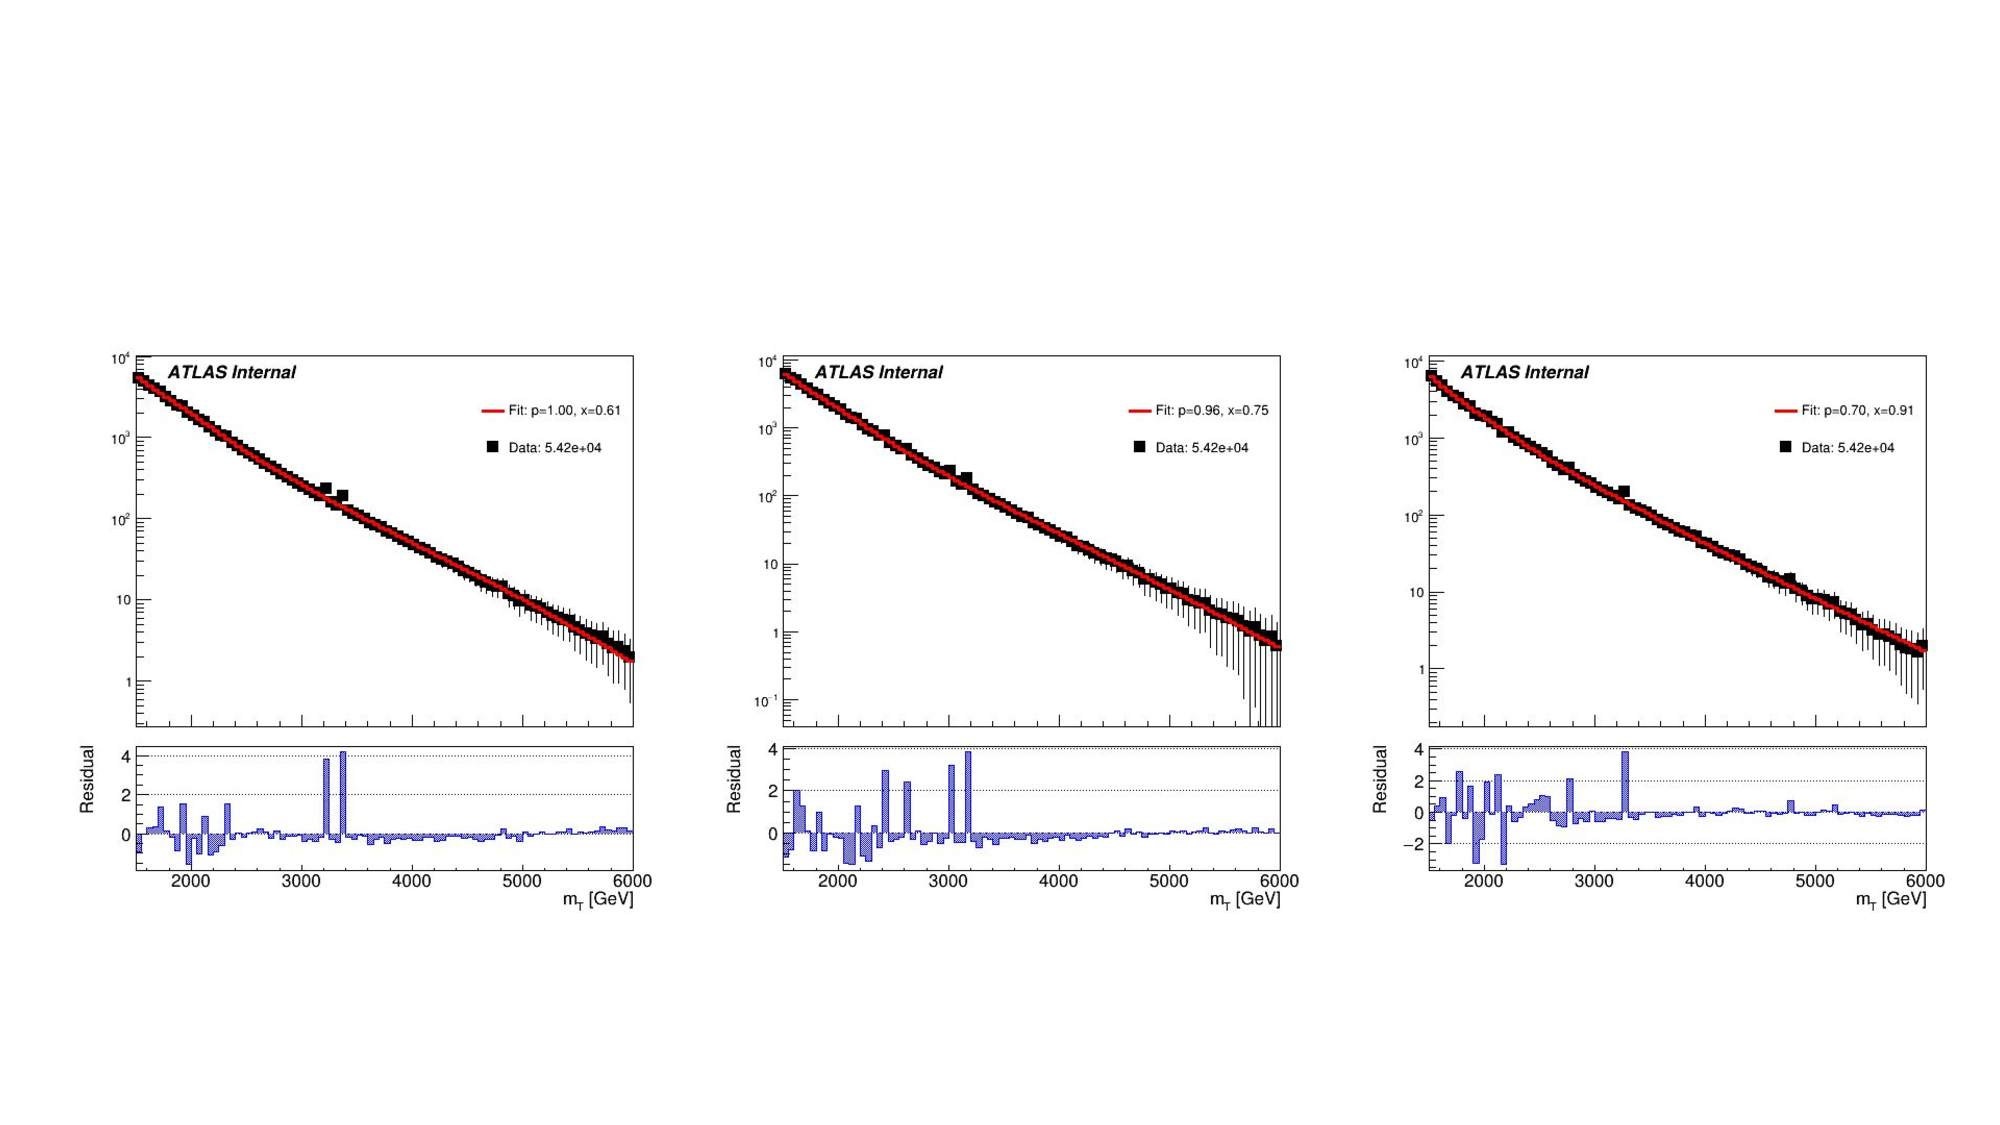
\includegraphics[width=0.95\textwidth]{figures/stats/bkgfit_mc}
    \caption{Background-only \mt~fits using representative MC in the CR (left), VR (middle), and SR (right).
    \label{fig:bkgfit_mc}}
\end{figure}

After verifying the background modeling in all analysis regions in simulation, it is tested in two data regions, the CR (low jet2width) and the VR (low ML score) which are orthogonal to the blinded SR.
Each \mt~histogram fit is obtained from randomly downsampling the original statistics in the CR/VR until a \textit{statistically identical} sample is obtained.
Three downsampled histograms are provided for each region, each with a random selection of events to match the expected SR event yields. 
Figure~\ref{fig:bkgfit_data} shows both of these regions, with high background only $p$-values indicating good compatibility.
For closure, Figure~\ref{fig:bkgfit_data_fullstats} shows the same fit performed to the full statistics CR and VR regions.
\begin{figure}[!htbp]
\centering
   %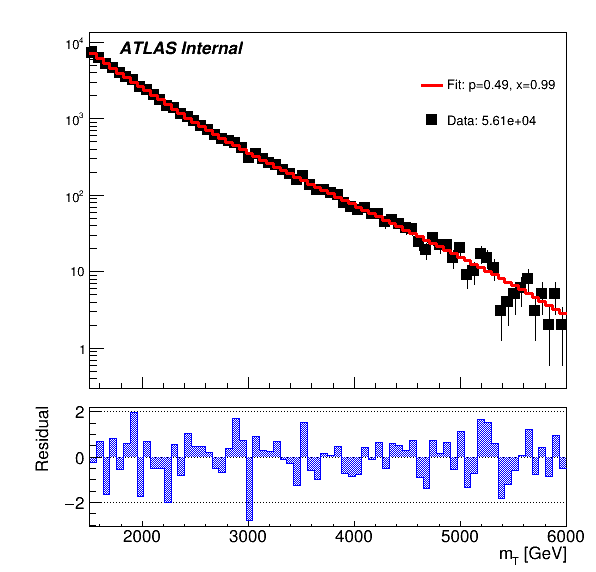
\includegraphics[width=0.32\textwidth]{figures/stats/dataDSfiveParFitChi2_CR0.png}
   %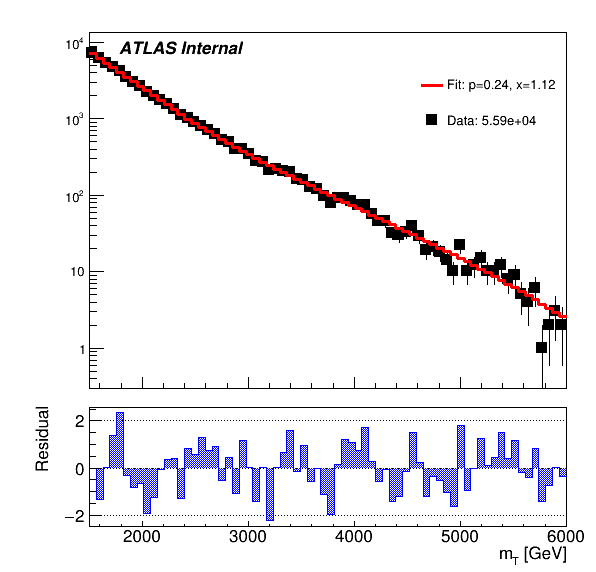
\includegraphics[width=0.32\textwidth]{figures/stats/dataDSfiveParFitChi2_CR1.png}
   %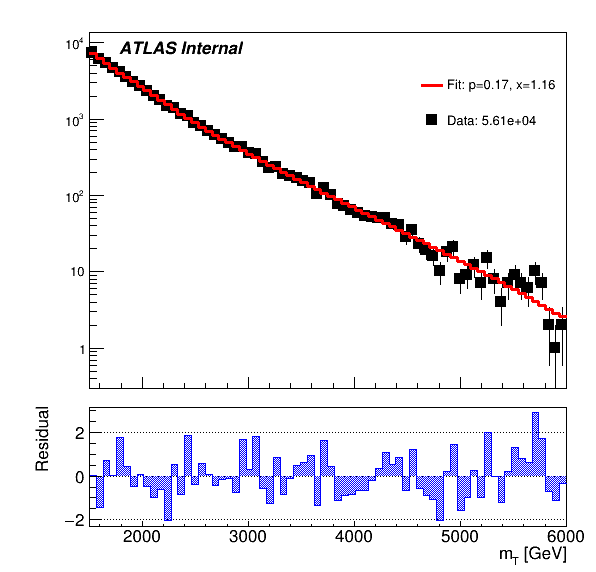
\includegraphics[width=0.32\textwidth]{figures/stats/dataDSfiveParFitChi2_CR2.png}
   %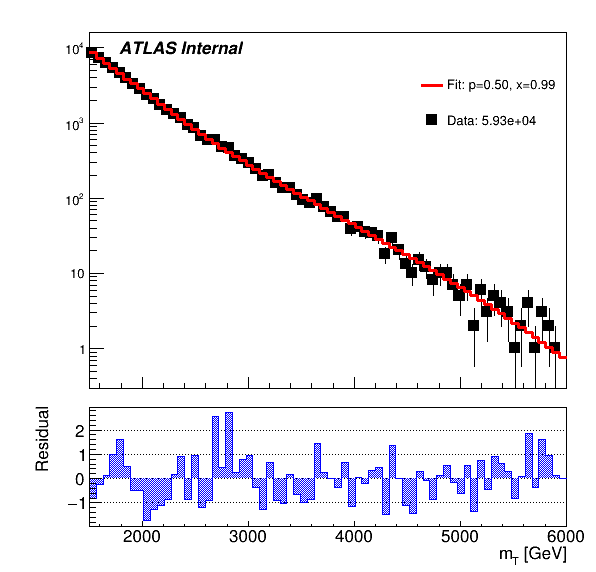
\includegraphics[width=0.32\textwidth]{figures/stats/dataDSfiveParFitChi2_VR0.png}
   %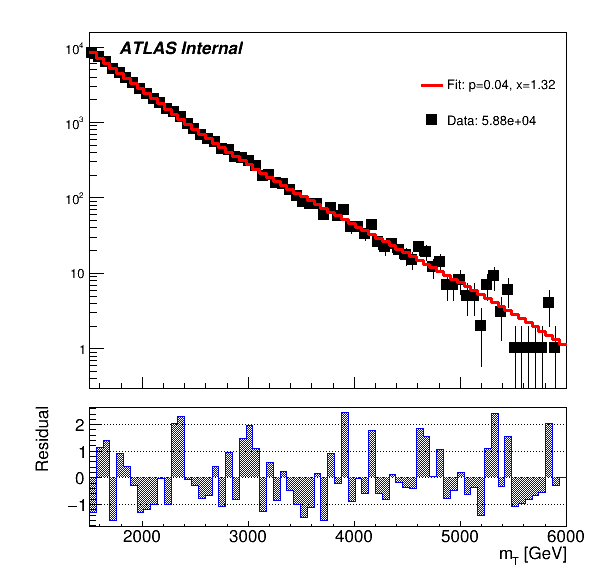
\includegraphics[width=0.32\textwidth]{figures/stats/dataDSfiveParFitChi2_VR1.png}
   %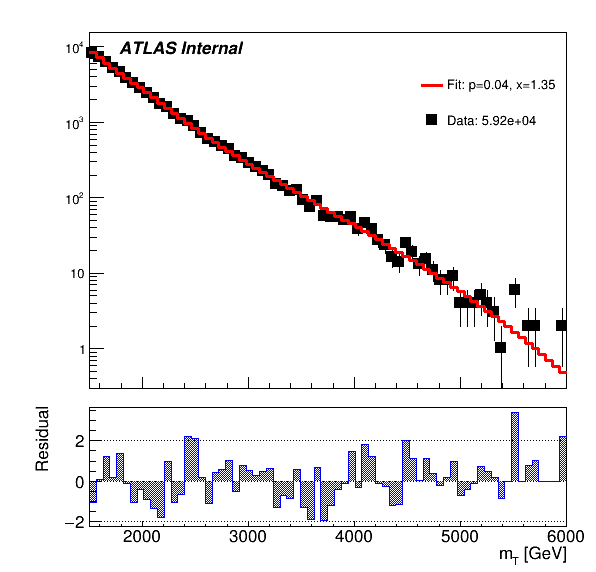
\includegraphics[width=0.32\textwidth]{figures/stats/dataDSfiveParFitChi2_VR2.png}
   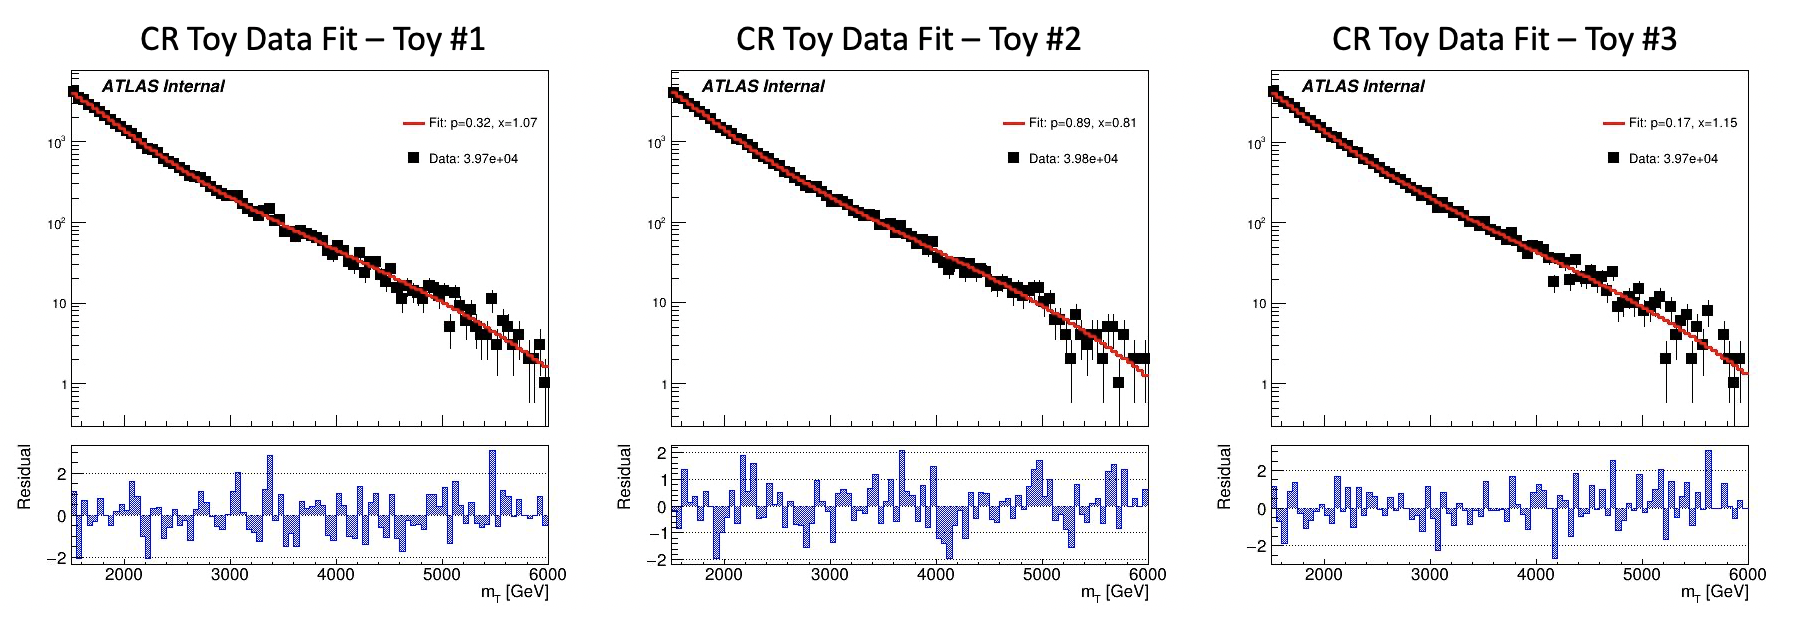
\includegraphics[width=0.92\textwidth]{figures/stats/bkgfit_data_cr}
   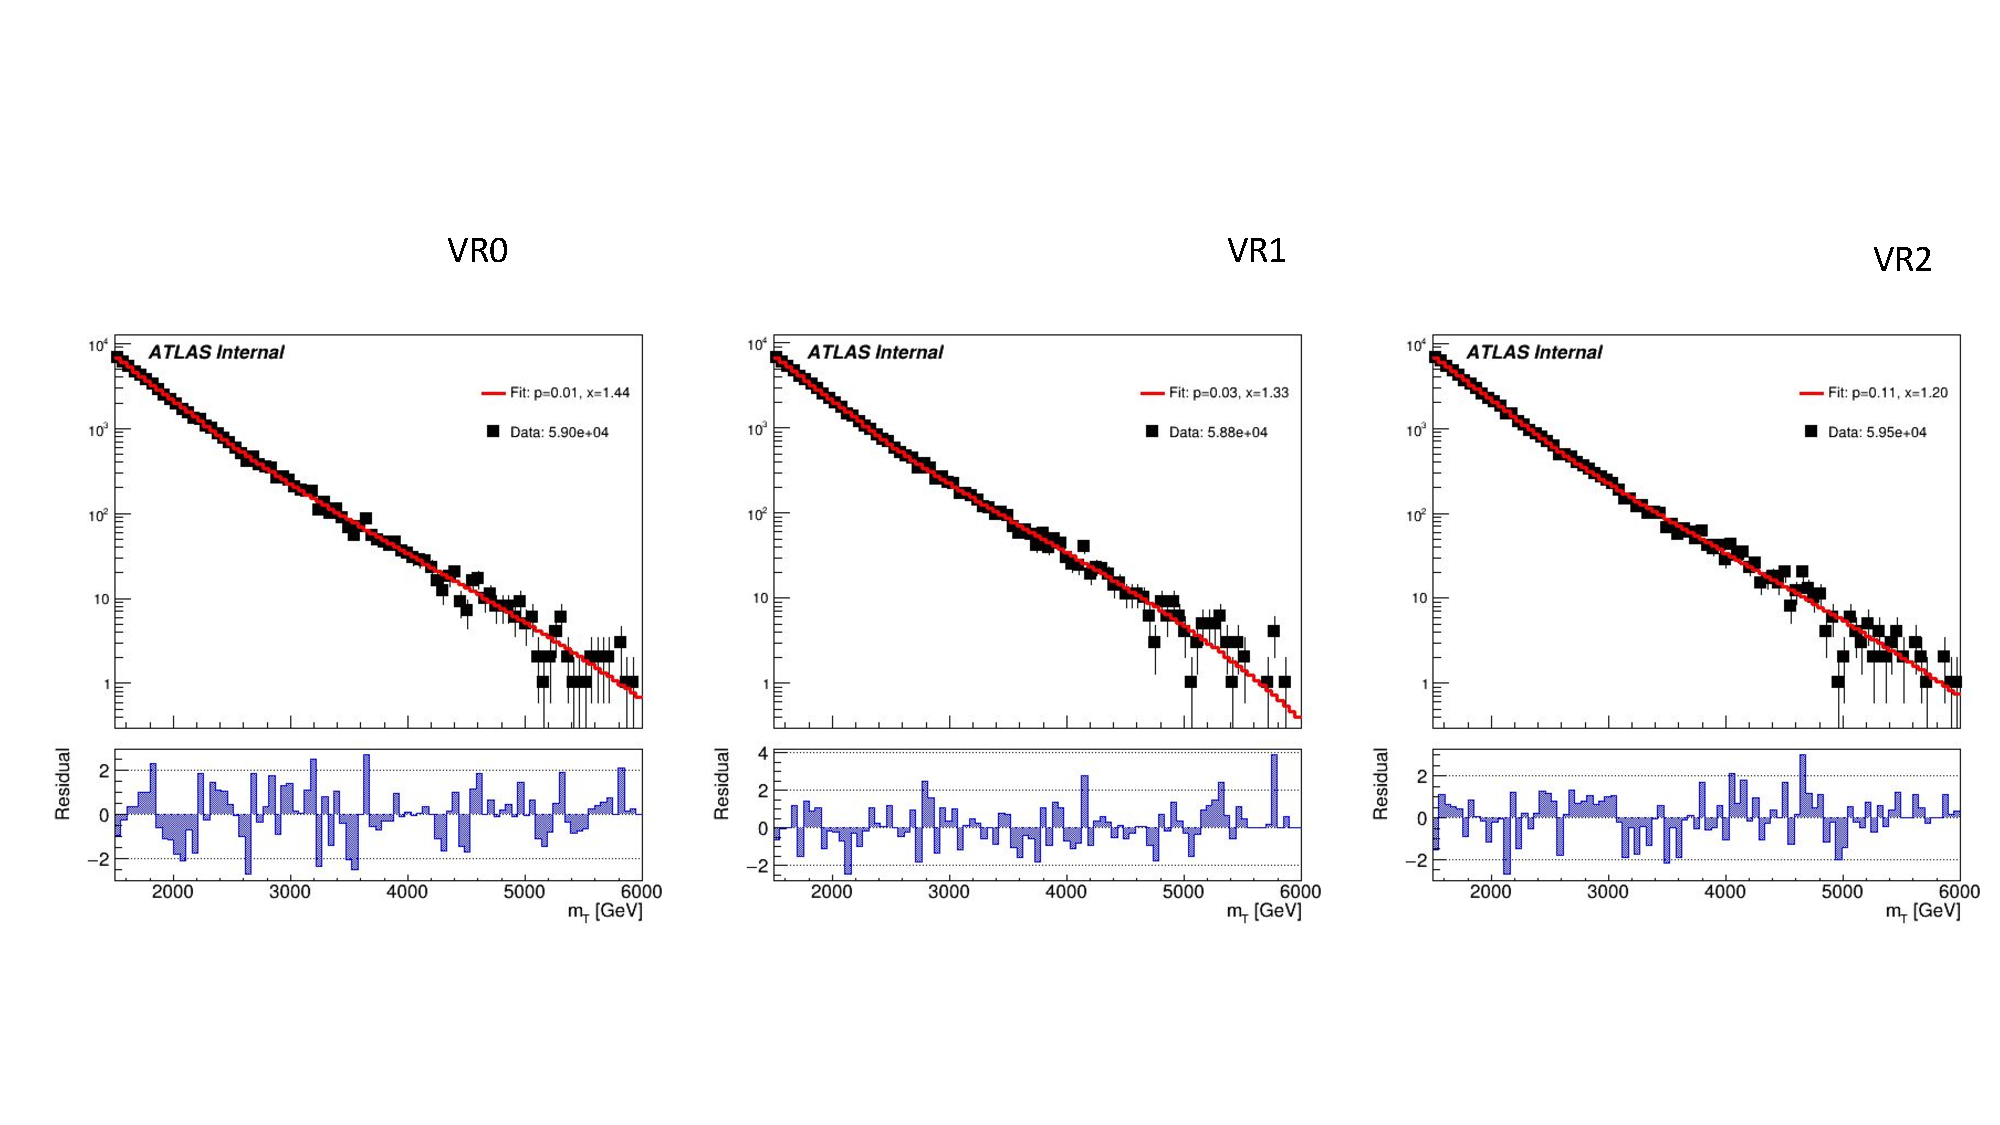
\includegraphics[width=0.92\textwidth]{figures/stats/bkgfit_data_vr}
    \caption{Background-only \mt~fits using data in orthogonal but statistically identical samples to the SR, obtained by downsampling the CR/VR statistics, for the CR (top) and VR (bottom).
    \label{fig:bkgfit_data}}
\end{figure}

\begin{figure}[!htbp]
\centering
   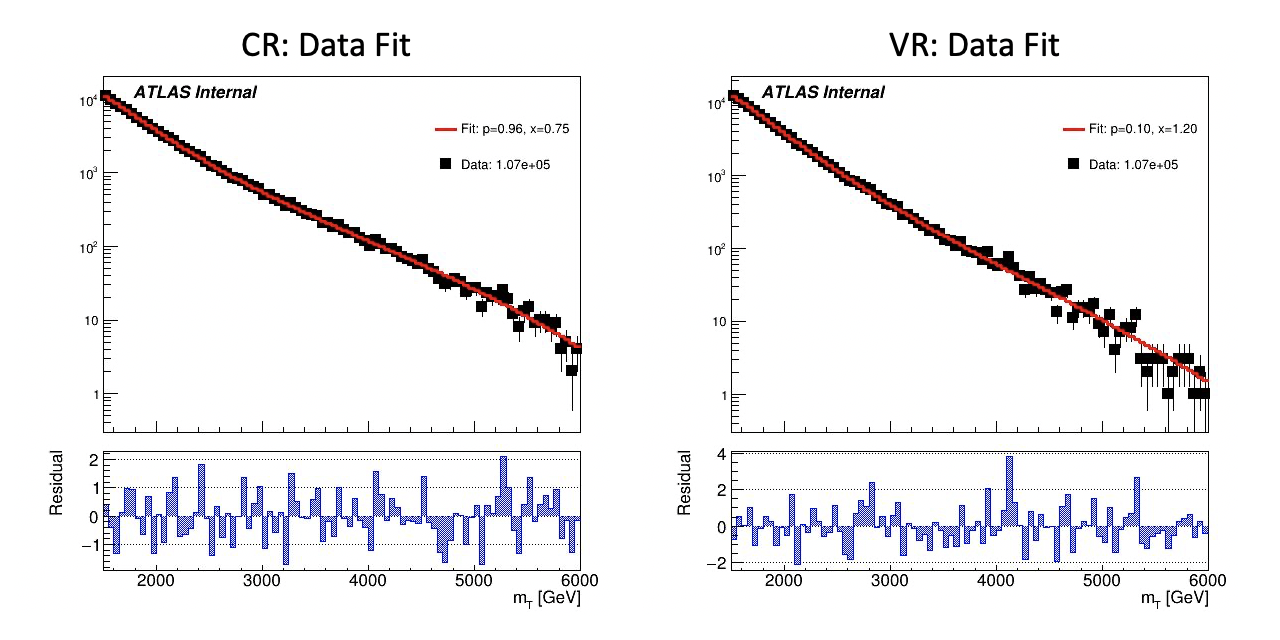
\includegraphics[width=0.82\textwidth]{figures/stats/bkgfit_data_fullstats}
    \caption{Background-only \mt~fits using data in the full statistics CR and VR regions.
    \label{fig:bkgfit_data_fullstats}}
\end{figure}

To further validate the fit in more instances, pseudo-data is created from the CR/VR data distributions. 
It is created following the Asimov prescription with smoothing to accommodate fluctuations in the high \mt~tail. 
The smoothing applied follows the procedure for functional decomposition described in Ref.~\cite{edgar2018functional}.
Figure~\ref{fig:smoothing} shows the impact of smoothing on the source data distribution in the CR.
Toys are then thrown from the smoothed distribution.
\begin{figure}[!htbp]
\centering
   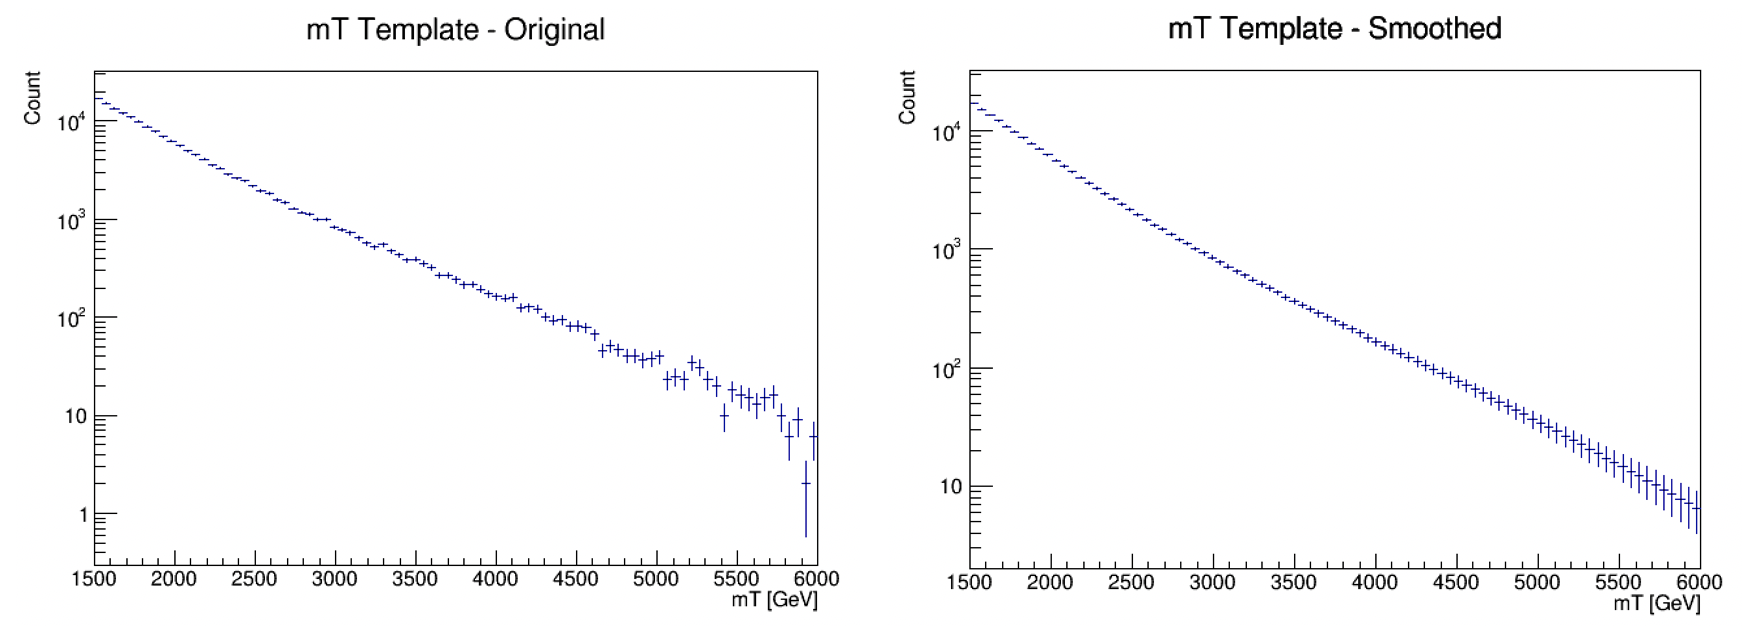
\includegraphics[width=0.85\textwidth]{figures/stats/smoothing}
    \caption{\mt~distribution in the data CR, before (left) and after (right) smoothing.
    \label{fig:smoothing}}
\end{figure}

Figure~\ref{fig:asimov_hist} shows the resulting p-values after an ensemble of 100 fits to varying pseudo-data distributions sourced from the data CR. 
A flat distribution is observed, indicating good statistical behavior.
\begin{figure}[!htbp]
\centering
   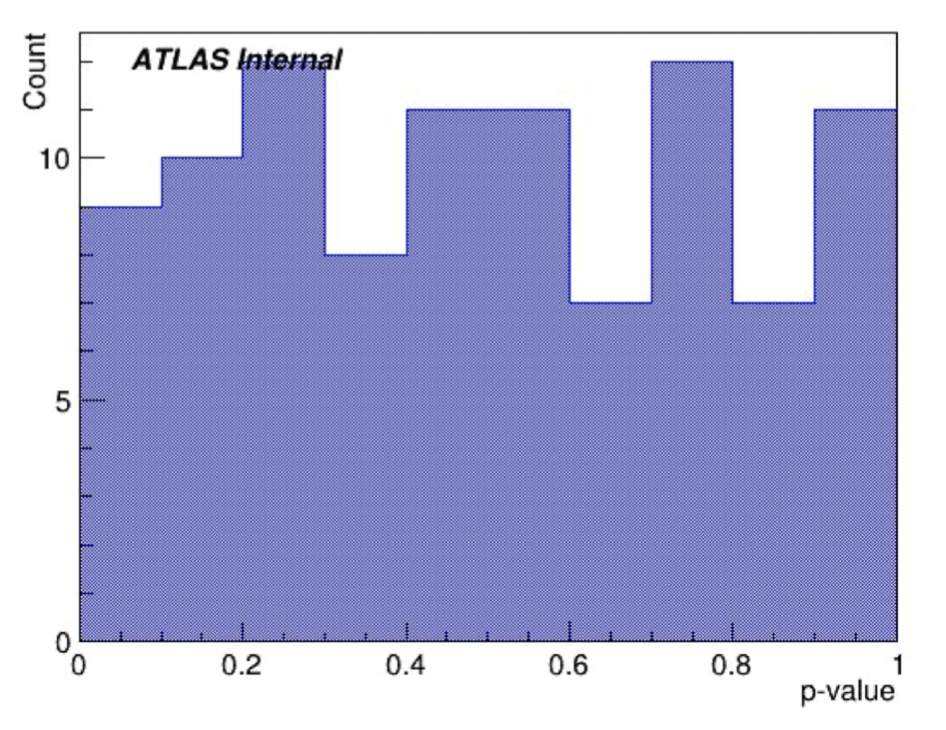
\includegraphics[width=0.45\textwidth]{figures/stats/asimov_cr_hist}
    \caption{$p$-value histograms from 500 fits to Asimov data in the CR. %, demonstrating a flat shape across p-value.
    \label{fig:asimov_hist}}
\end{figure}




%------------------------------------------------- 
\subsubsection{Signal + Background Fits}
\label{subsec:fit_splusb}

Figure~\ref{fig:splusb_ex} shows some examples of S+B fits on the background-only distribution for a variety of signal hypotheses across the (\rinv, mass) grid.
\begin{figure}[!htbp]
\centering
   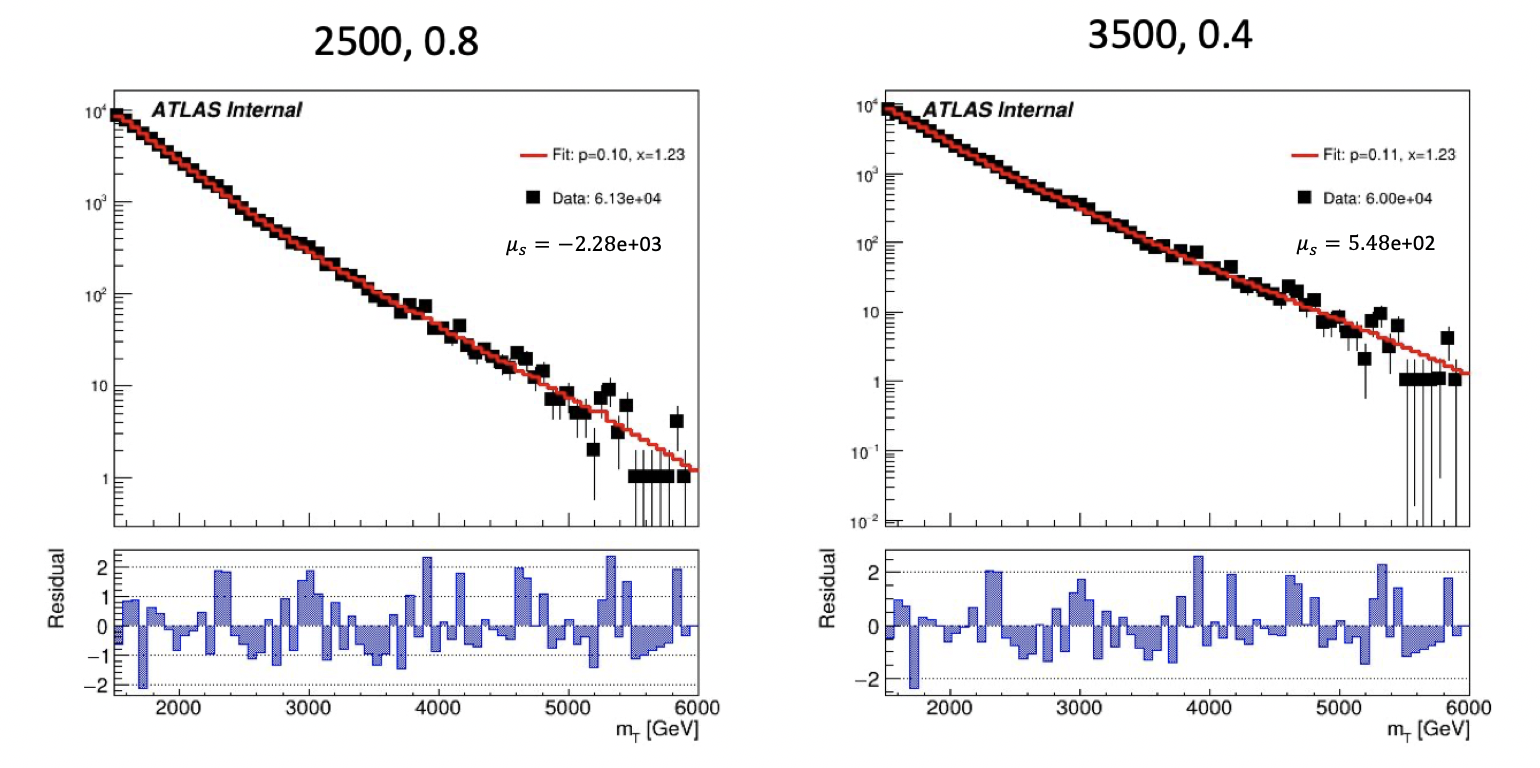
\includegraphics[width=0.8\textwidth]{figures/stats/splusb_ex1}
   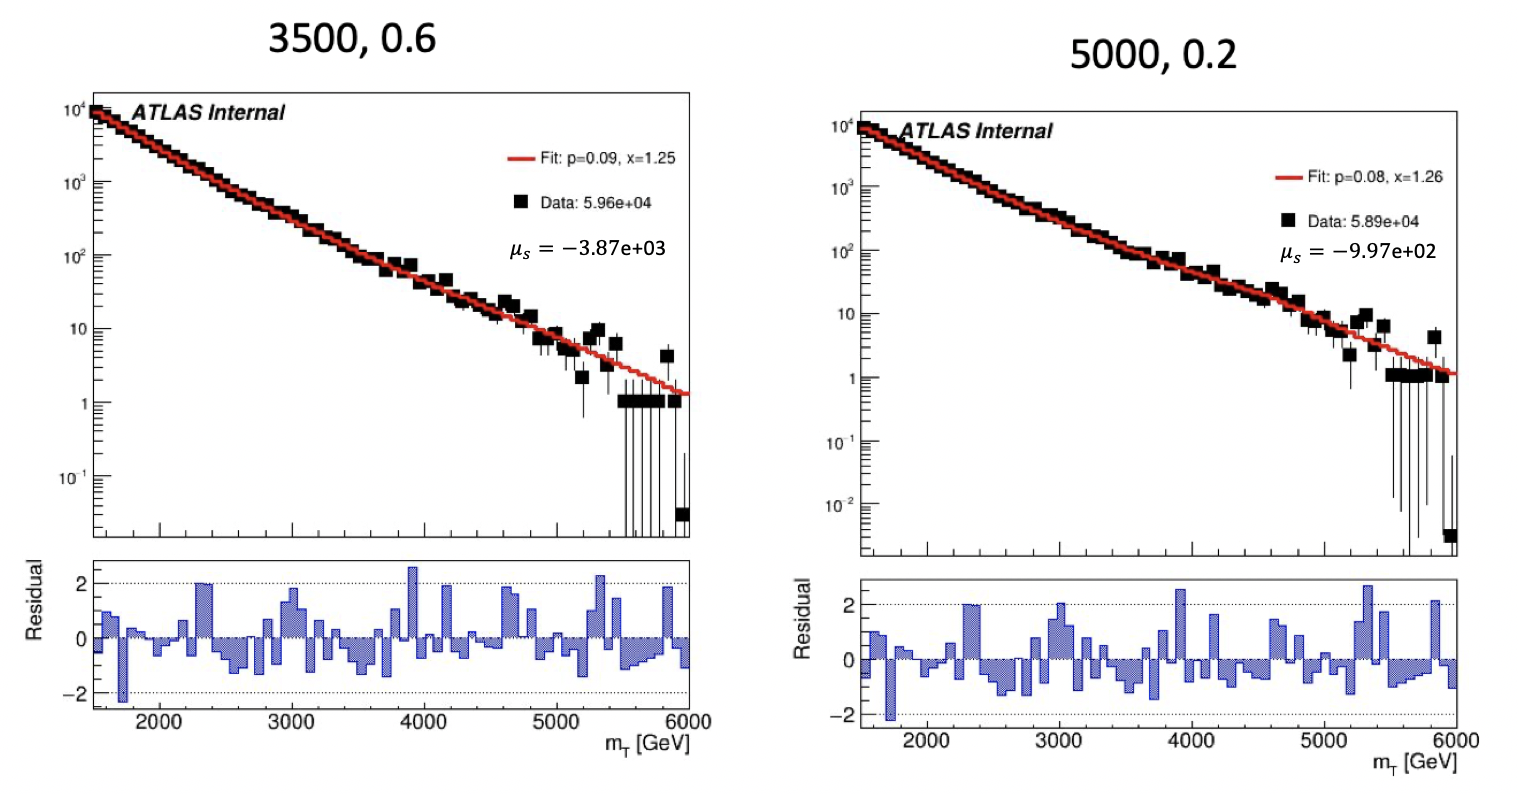
\includegraphics[width=0.8\textwidth]{figures/stats/splusb_ex2}
    \caption{Example S+B fits on background only spectrum (without systematics) for a variety of signal points.
    \label{fig:splusb_ex}}
\end{figure}


\paragraph{Spurious Signal}

The spurious signal fits are done using S+B fits on signal-depleted regions. 
These fits performed in pseudodata derived from a smoothed CR template are used to calculate the spurious signal uncertainty, as described in Section~\ref{sec:syst}.

\clearpage


\paragraph{Signal Injection in CR Template}

Figure~\ref{fig:splusb_sigInj} shows an example of an injected signal into the exclusion region \mt~spectrum, and the ability of the fit framework to accurately fit the number of signal events.
\begin{figure}[!htbp]
\centering
   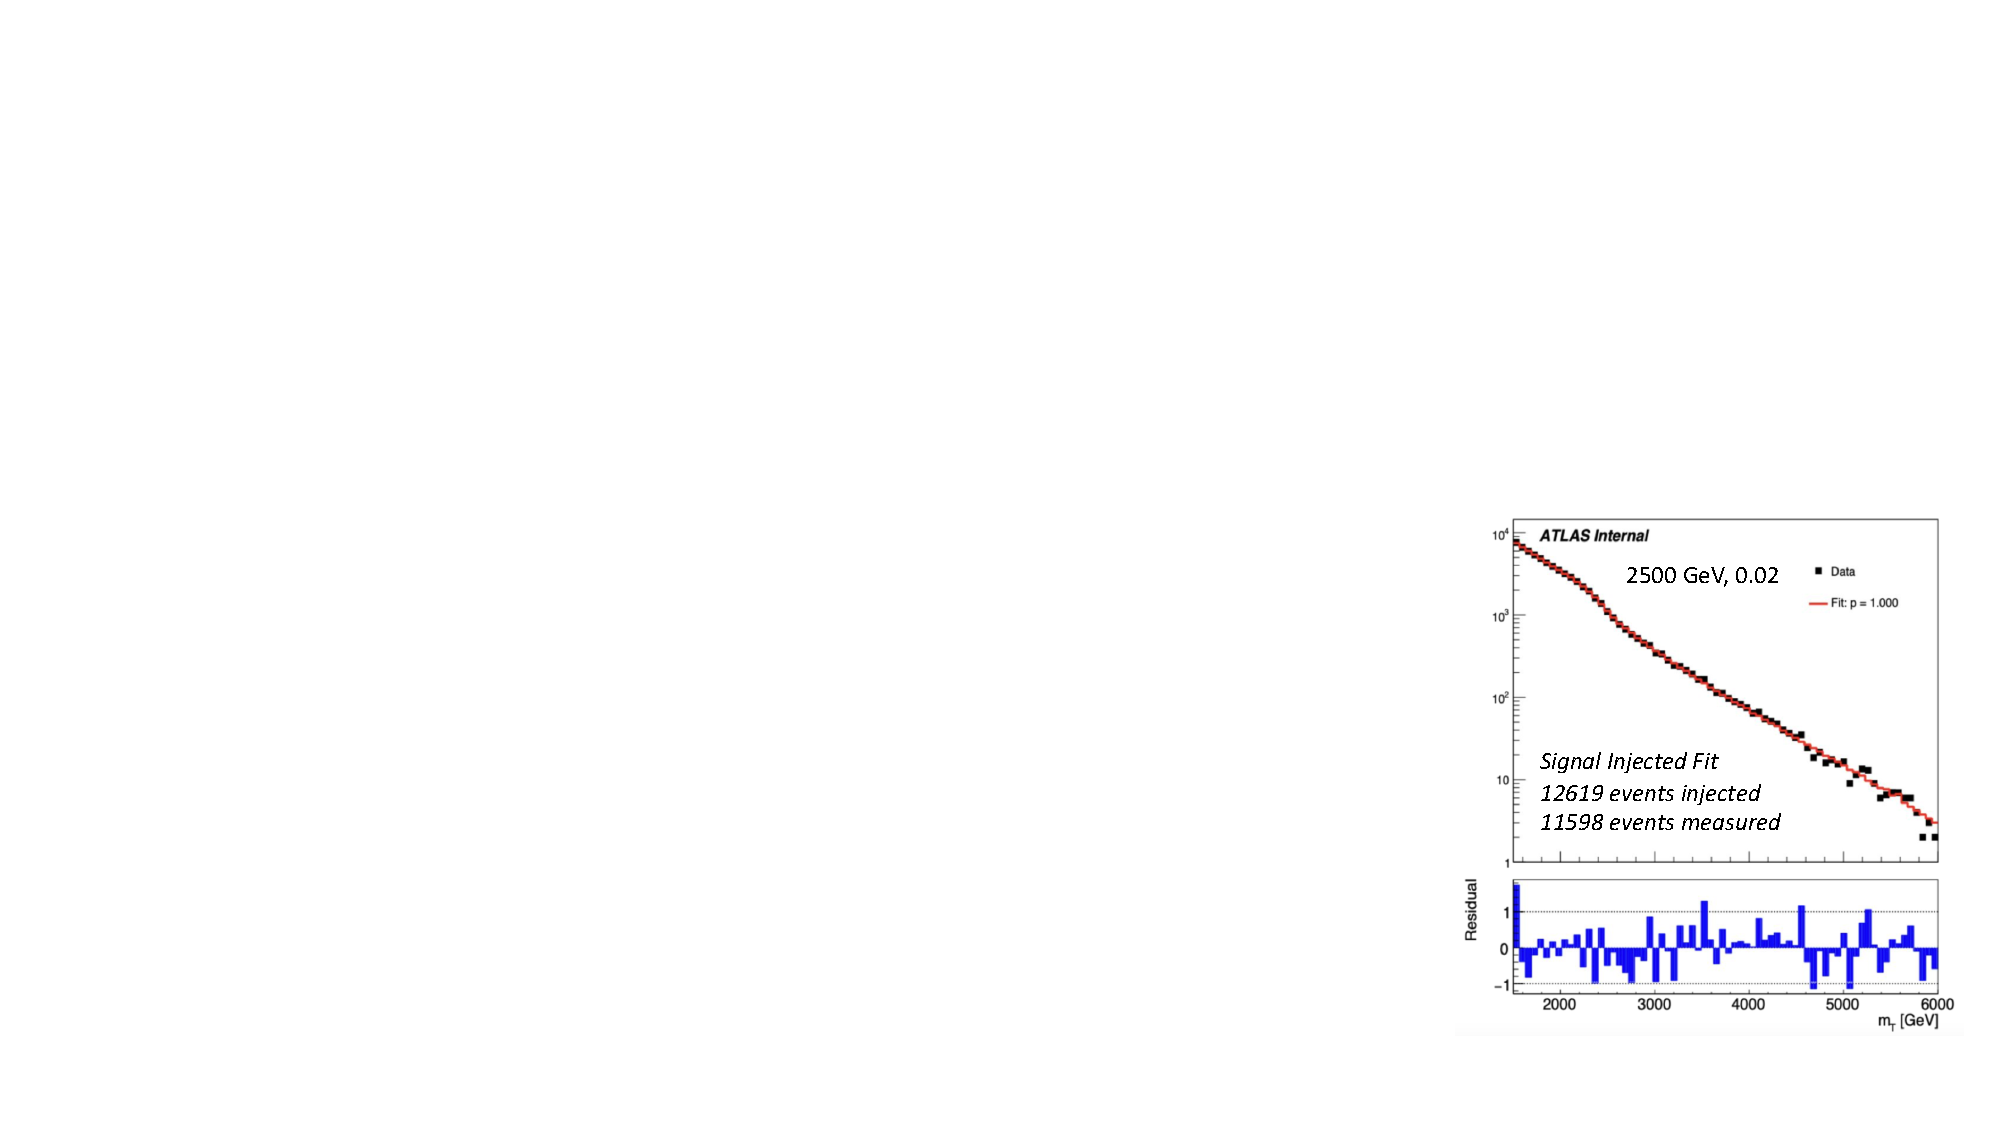
\includegraphics[width=0.6\textwidth]{figures/stats/splusb_sigInj}
    \caption{Example S+B fits on a background \mt~spectrum with injected signal from the point (2500 GeV, \rinv=0.2).
    \label{fig:splusb_sigInj}}
\end{figure}

Figure~\ref{fig:siginj_linearity} shows the linearity of the fitted signal as a function of the size of the injected signal, for all 4 \rinv~categories and several Z' masses.
No uncertainties on the signal model are included.
These fits are done in a single template of the CR, making the fitted signal prone to fluctuations in the underlying template, motivating the use of toys to better capture the behavior of the S+B fit in finding a signal.
\begin{figure}[!htbp]
\centering
   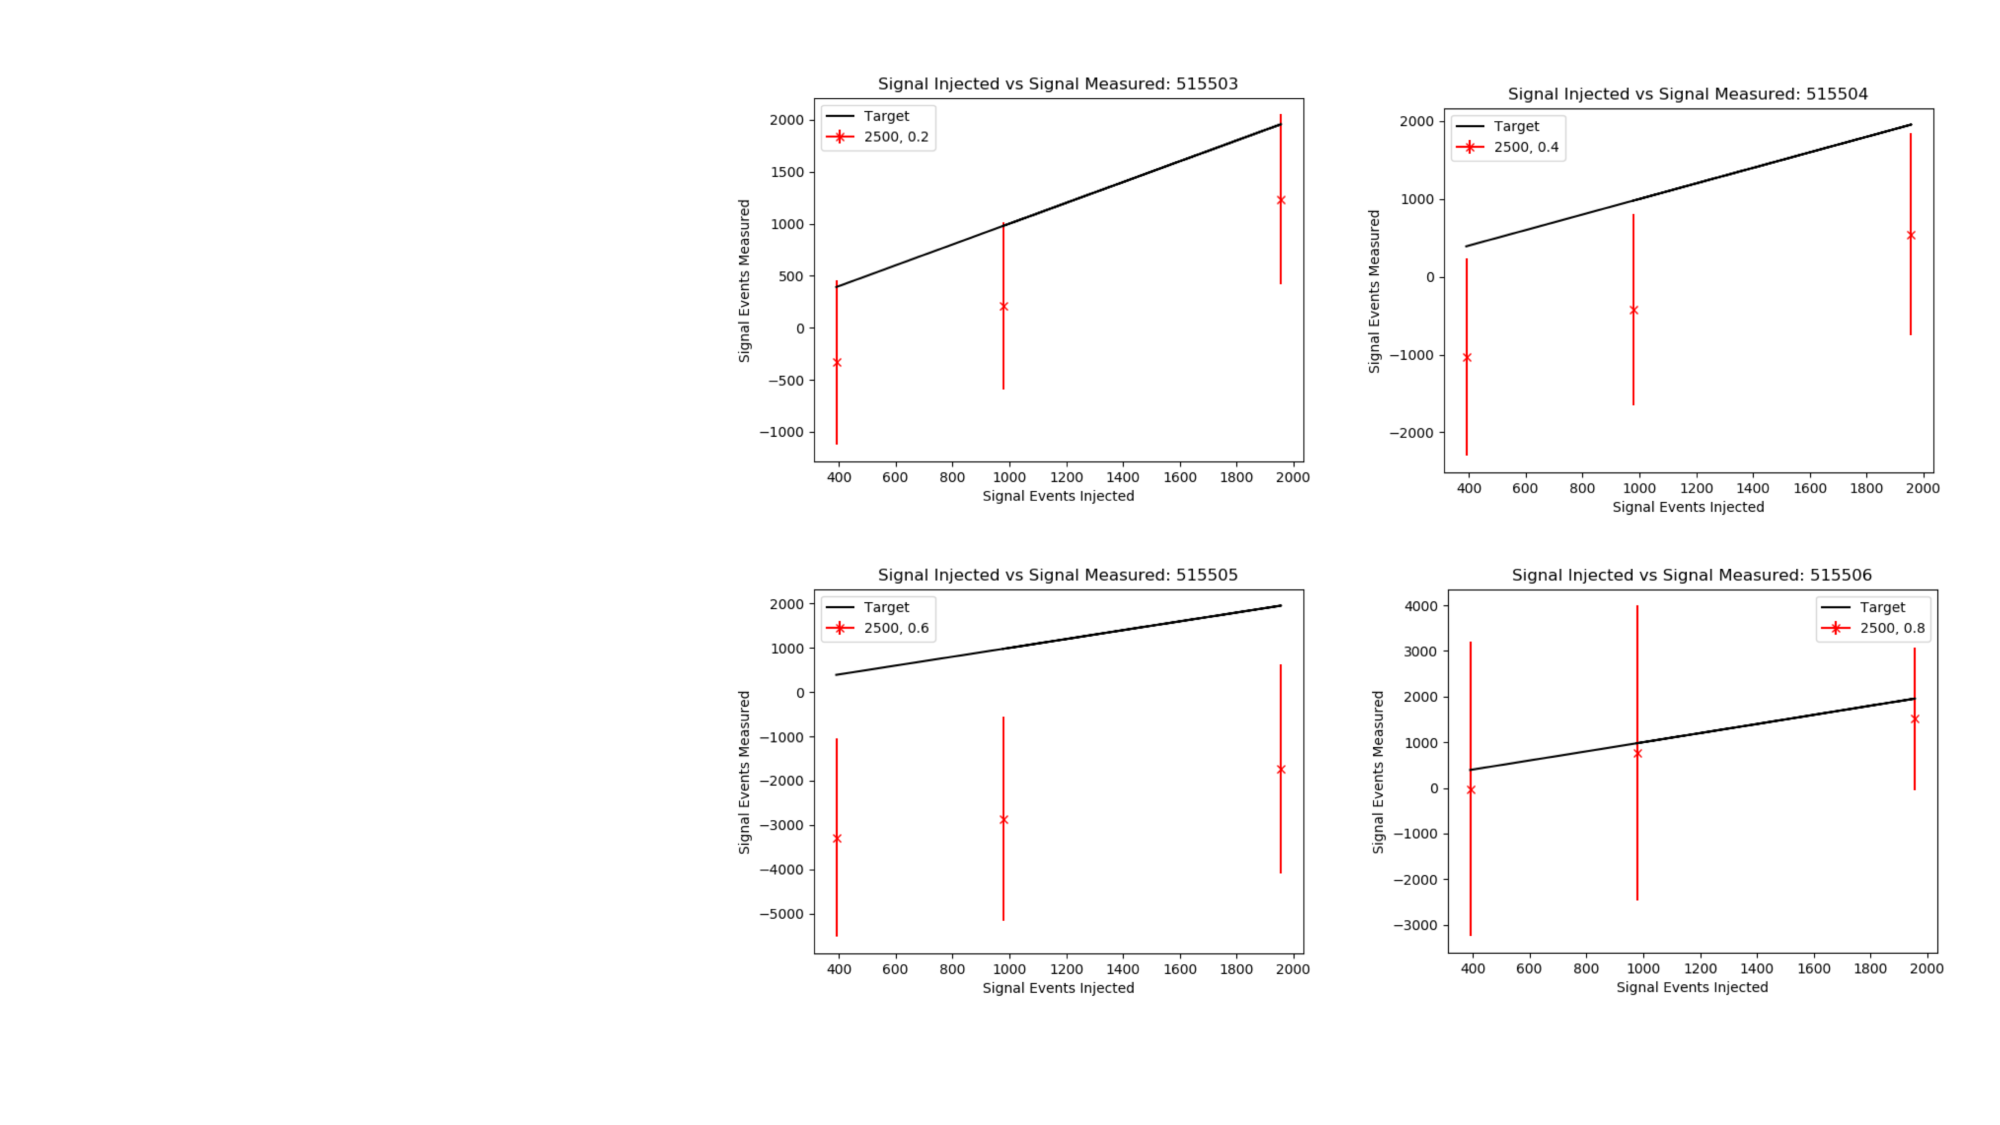
\includegraphics[width=0.6\textwidth]{figures/stats/siginj_m2500}
   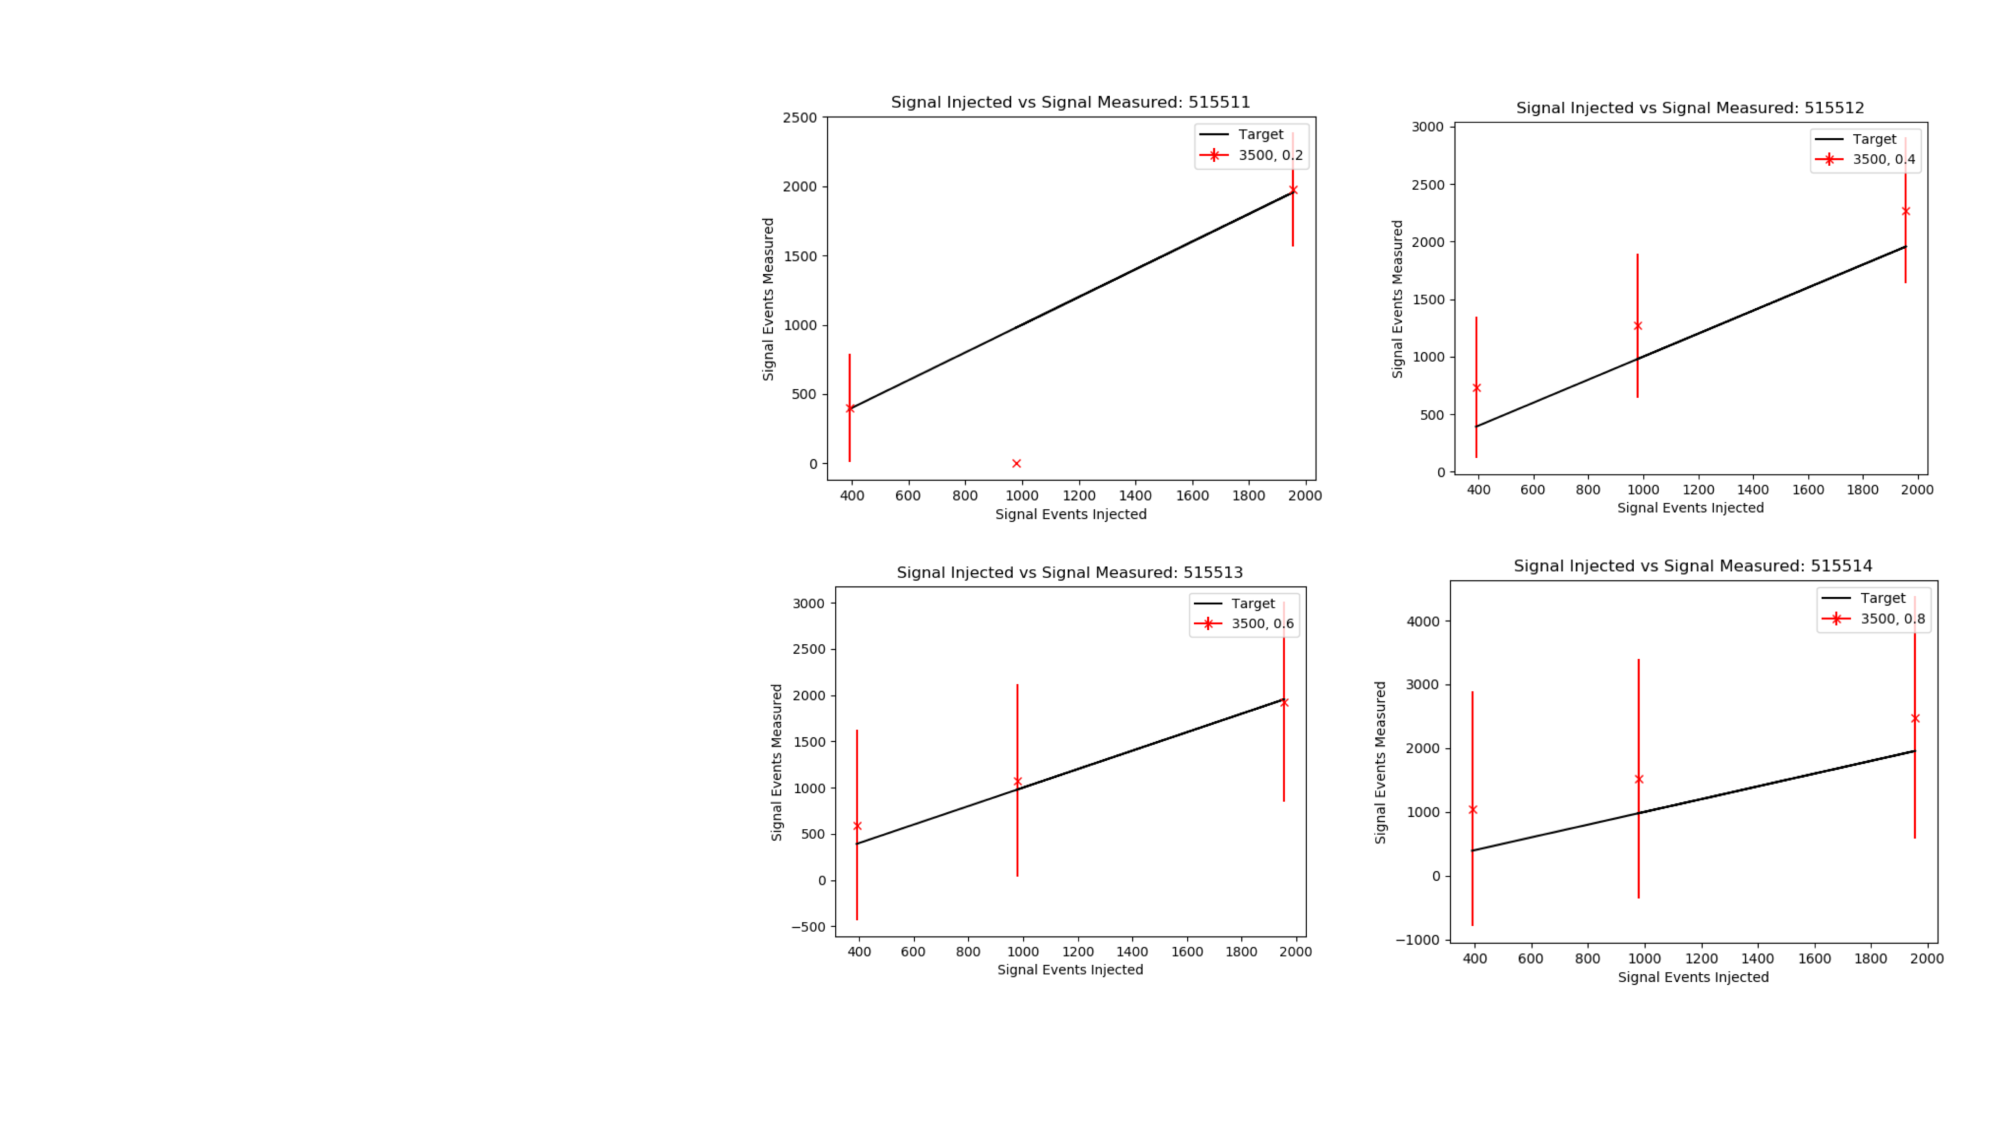
\includegraphics[width=0.6\textwidth]{figures/stats/siginj_m3500}
   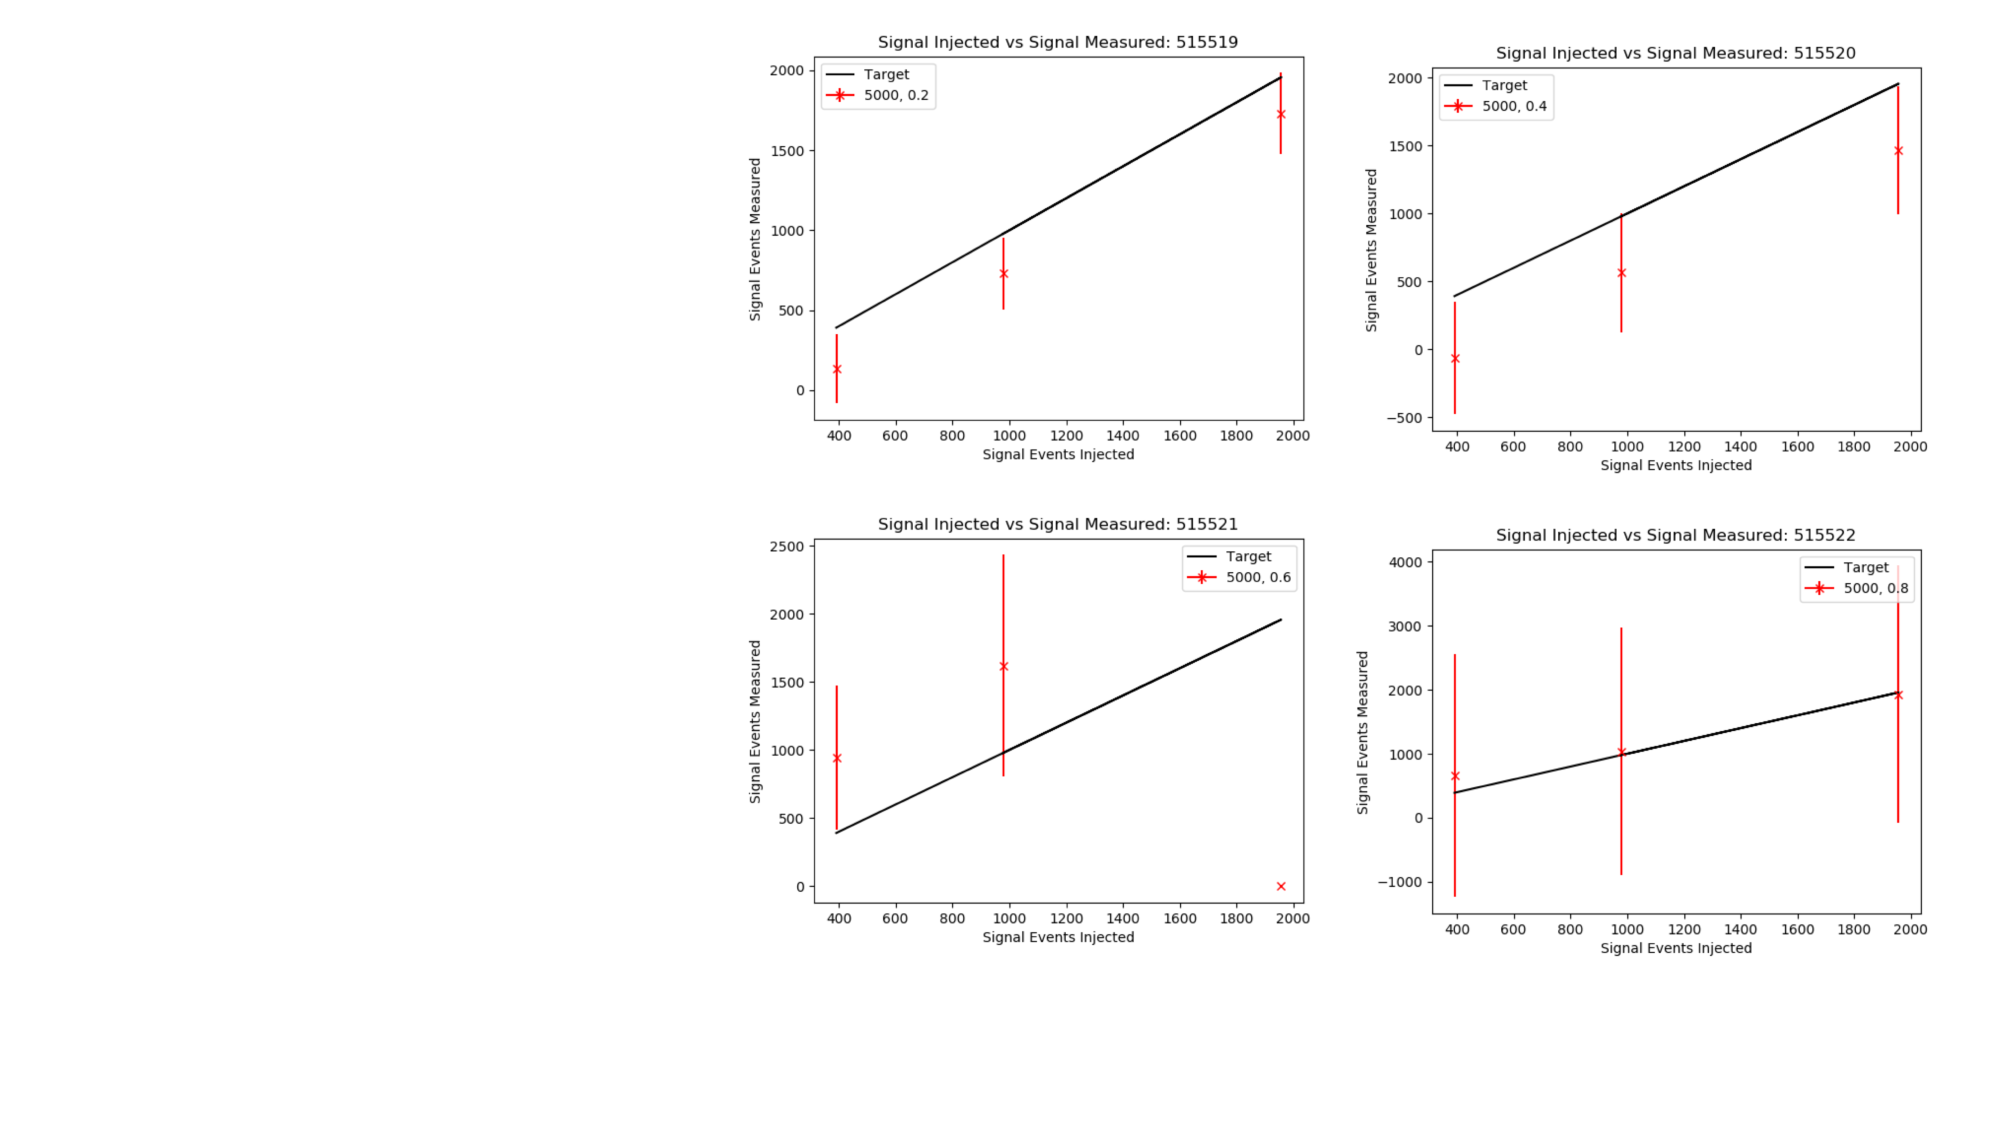
\includegraphics[width=0.6\textwidth]{figures/stats/siginj_m5000}
   \caption{Linearity of fitted vs. injected signal across \mt, for signal points with \rinv=0.2, 0.4, 0.6, and 0.8, with several Z' masses (2500 GeV, 3500 GeV, and 5000 GeV top to bottom) for a single CR template with no systematics.
    \label{fig:siginj_linearity}}
\end{figure}

\paragraph{Signal Injection in Asimov Data}
To better understand the correlations of fit errors in the above single-template injection test and avoid drawing conclusions from a single scenario, signal injection tests using Asimov data will be performed before unblinding. 
Criteria for this check are adapted from the Run 2 dijet TLA analysis~\footnote{\url{https://cds.cern.ch/record/2632454}, Section 10.4}.
50 Asimov trials are run for represenative signal points across Z' mass and \rinv.
Specifically, we will take the difference between fitted and injected signal events as a spurious signal and require it to be less than 10\% of the original injected signal yield, or its absolute value to be less than 50\% of the fitted signal RMS:
\begin{equation}
\label{eq:spursig}
S_{\text{spur}} = S_{\text{fit}} - S_{\text{inj}} < 0.1S_{\text{inj}} \ \text{OR} < 0.5\sigma_{\text{fit}}
\end{equation}

%Bias within the Asimov signal injection test could indicate a lack of sufficient normalization uncertainties on the signal model. 
%In the event of systematic mismeasurement in signal injection, the spurious signal uncertainty as derived from Loose-not-tight or additional uncertainties will be considered.

Figure~\ref{fig:siginj_asimov} provides tabular results of these tests, assessing both $S_{\text{spur}}$ from Equation~\ref{eq:spursig}.
Figure~\ref{fig:siginj_asimov_check} displays the measured S$_{\text{spur}}$/$\sigma_\text{fit}$ for each signal point to assess the criterion from Equation~\ref{eq:spursig}.
We find that all but 1 of the tested signal points and signal injection sizes (m$_{Z'}$ = 4000 GeV, \rinv=0.2 at 5$\sigma$ significance) pass the criteria in Equation~\ref{eq:spursig}. %, and that the signal injection tests pass all required criteria.
While (m$_{Z'}$ = 4000 GeV, \rinv=0.2) generally gives the highest S$_{\text{spur}}$ of all points, the one injected size that violates the test criterion is close to 0.5 and within a trend shared by all points. 
\begin{figure}[!htbp]
\centering
   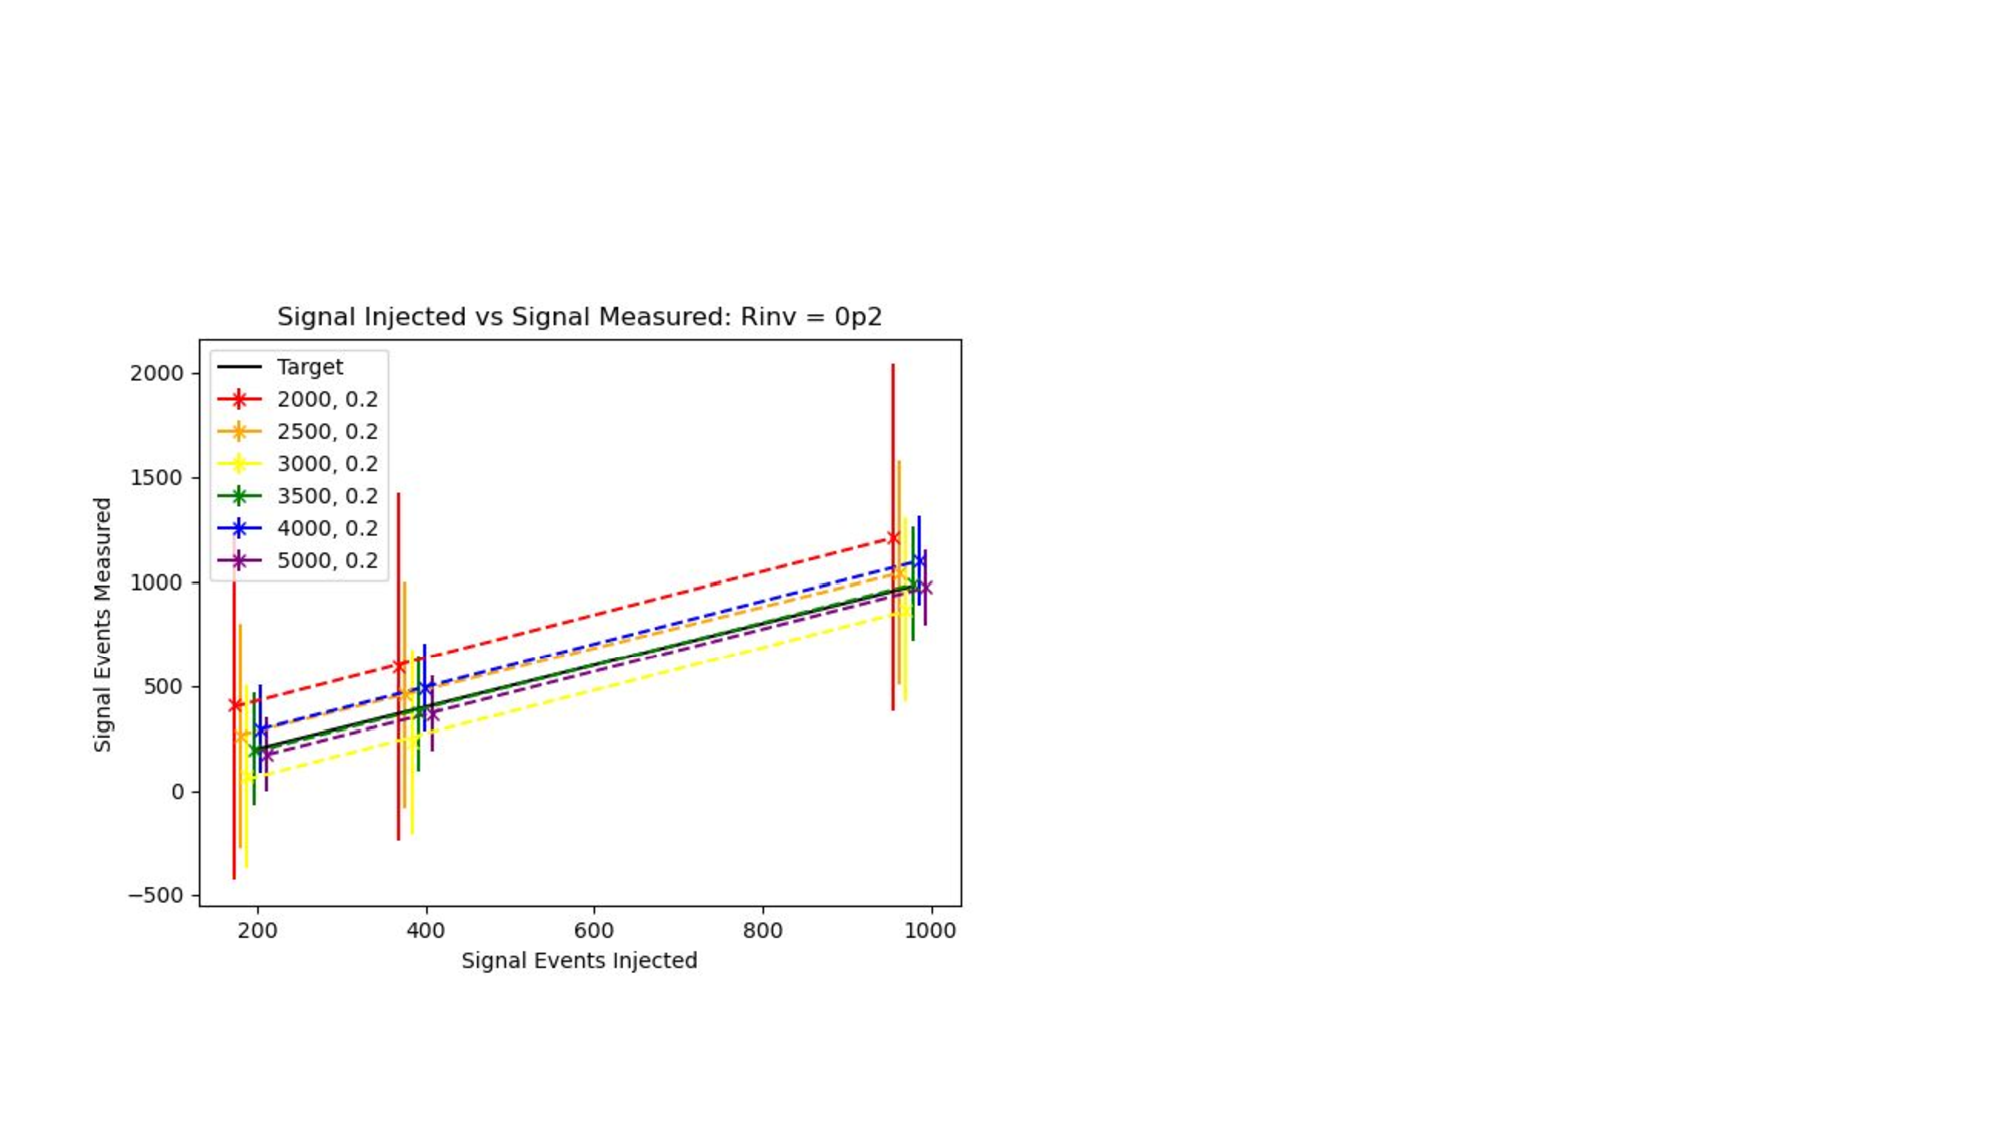
\includegraphics[width=0.45\textwidth]{figures/stats/siginj_asimov_02}
   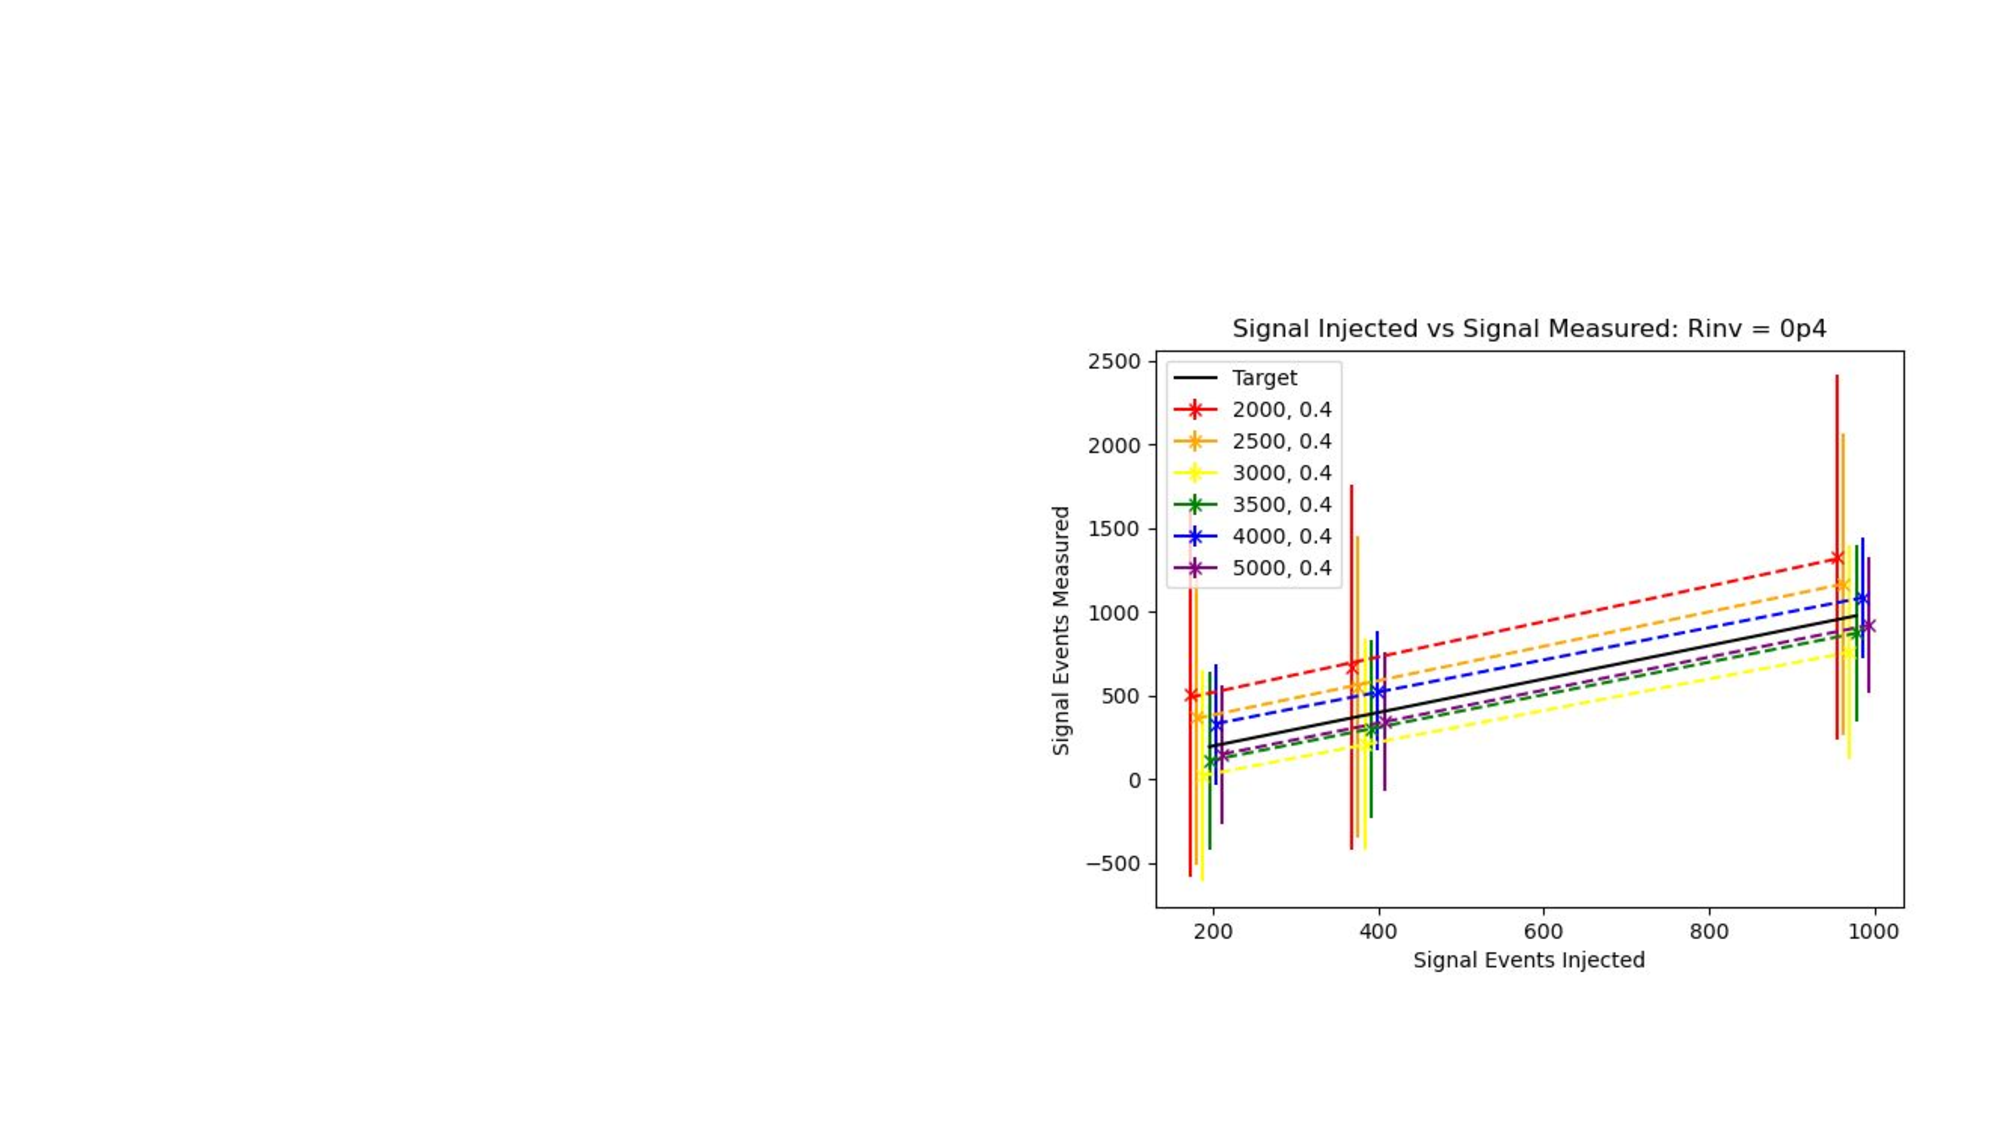
\includegraphics[width=0.45\textwidth]{figures/stats/siginj_asimov_04}
   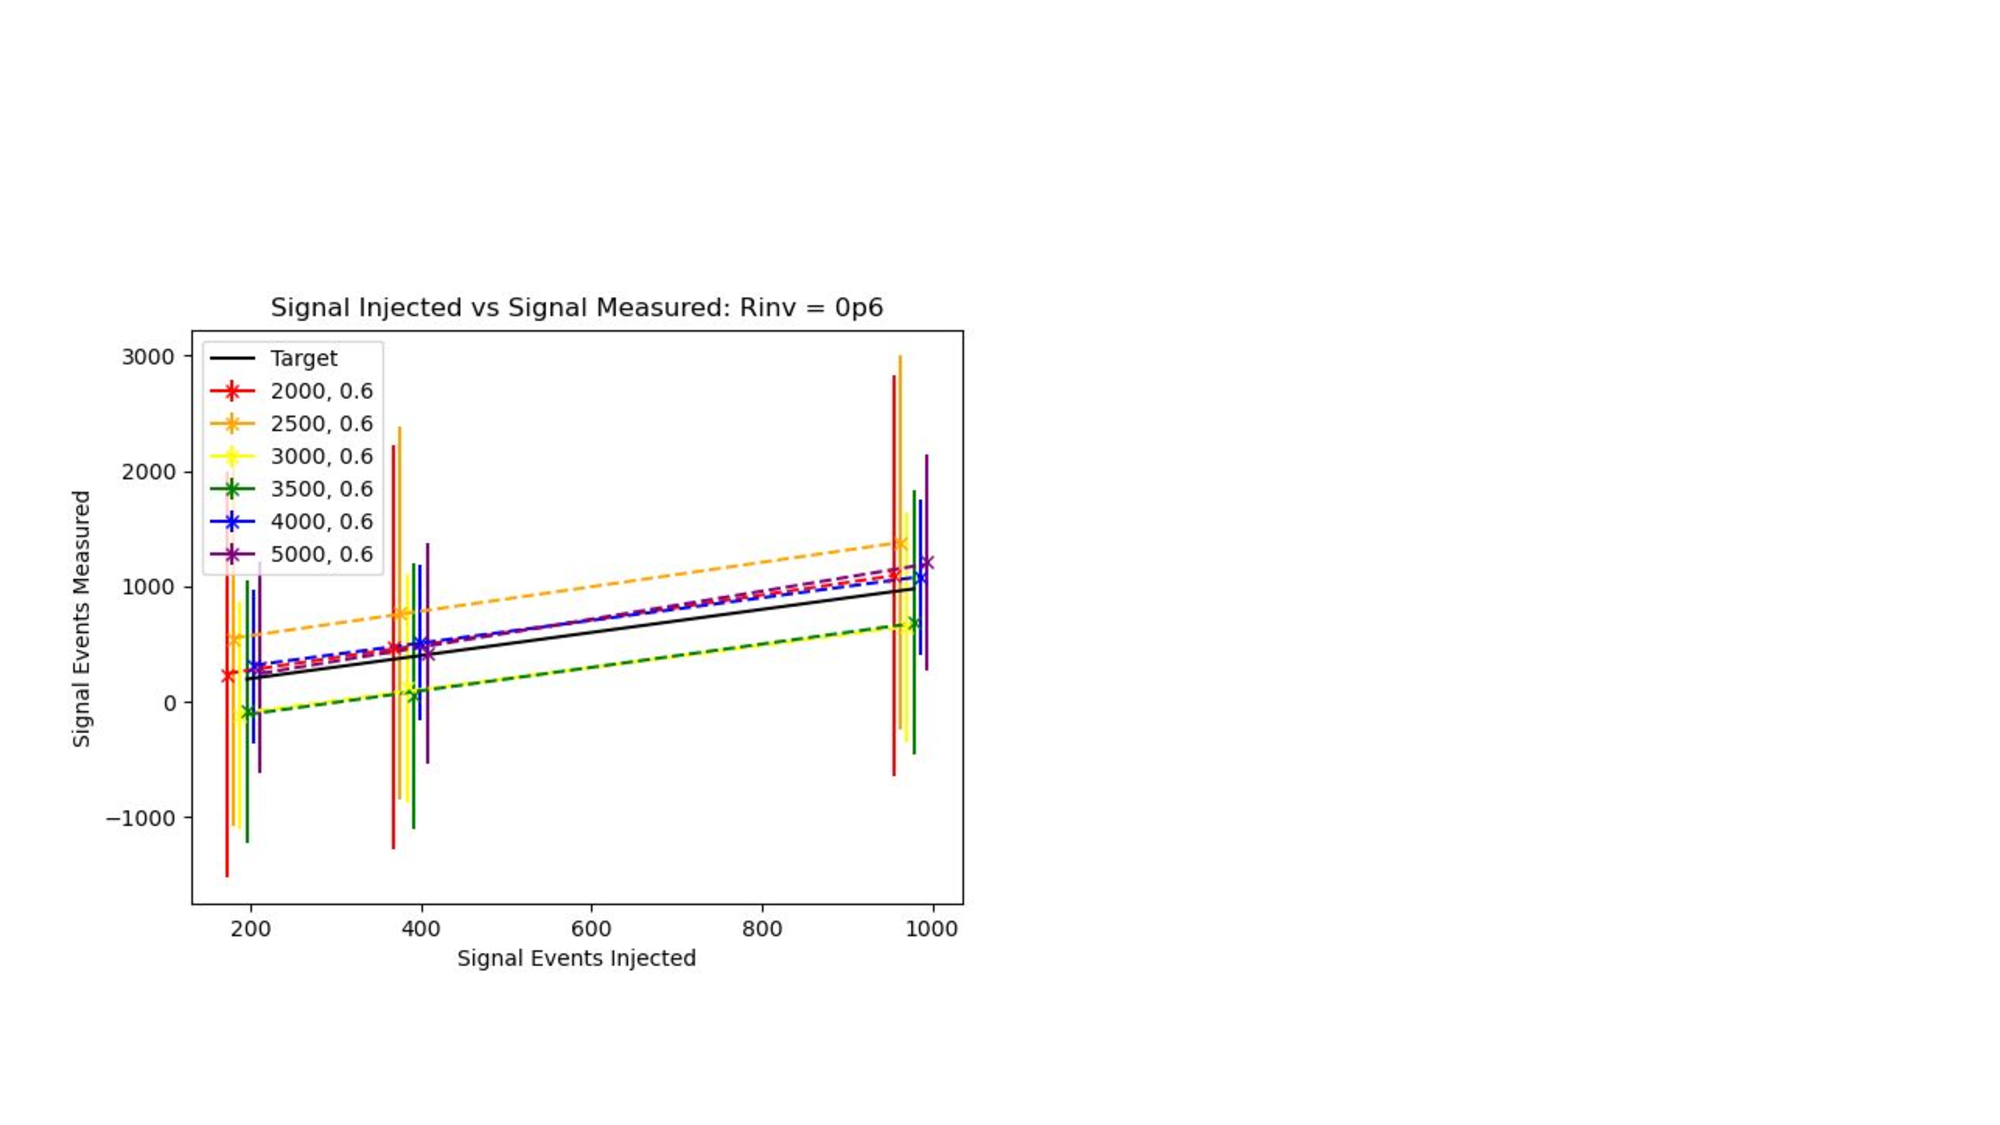
\includegraphics[width=0.45\textwidth]{figures/stats/siginj_asimov_06}
   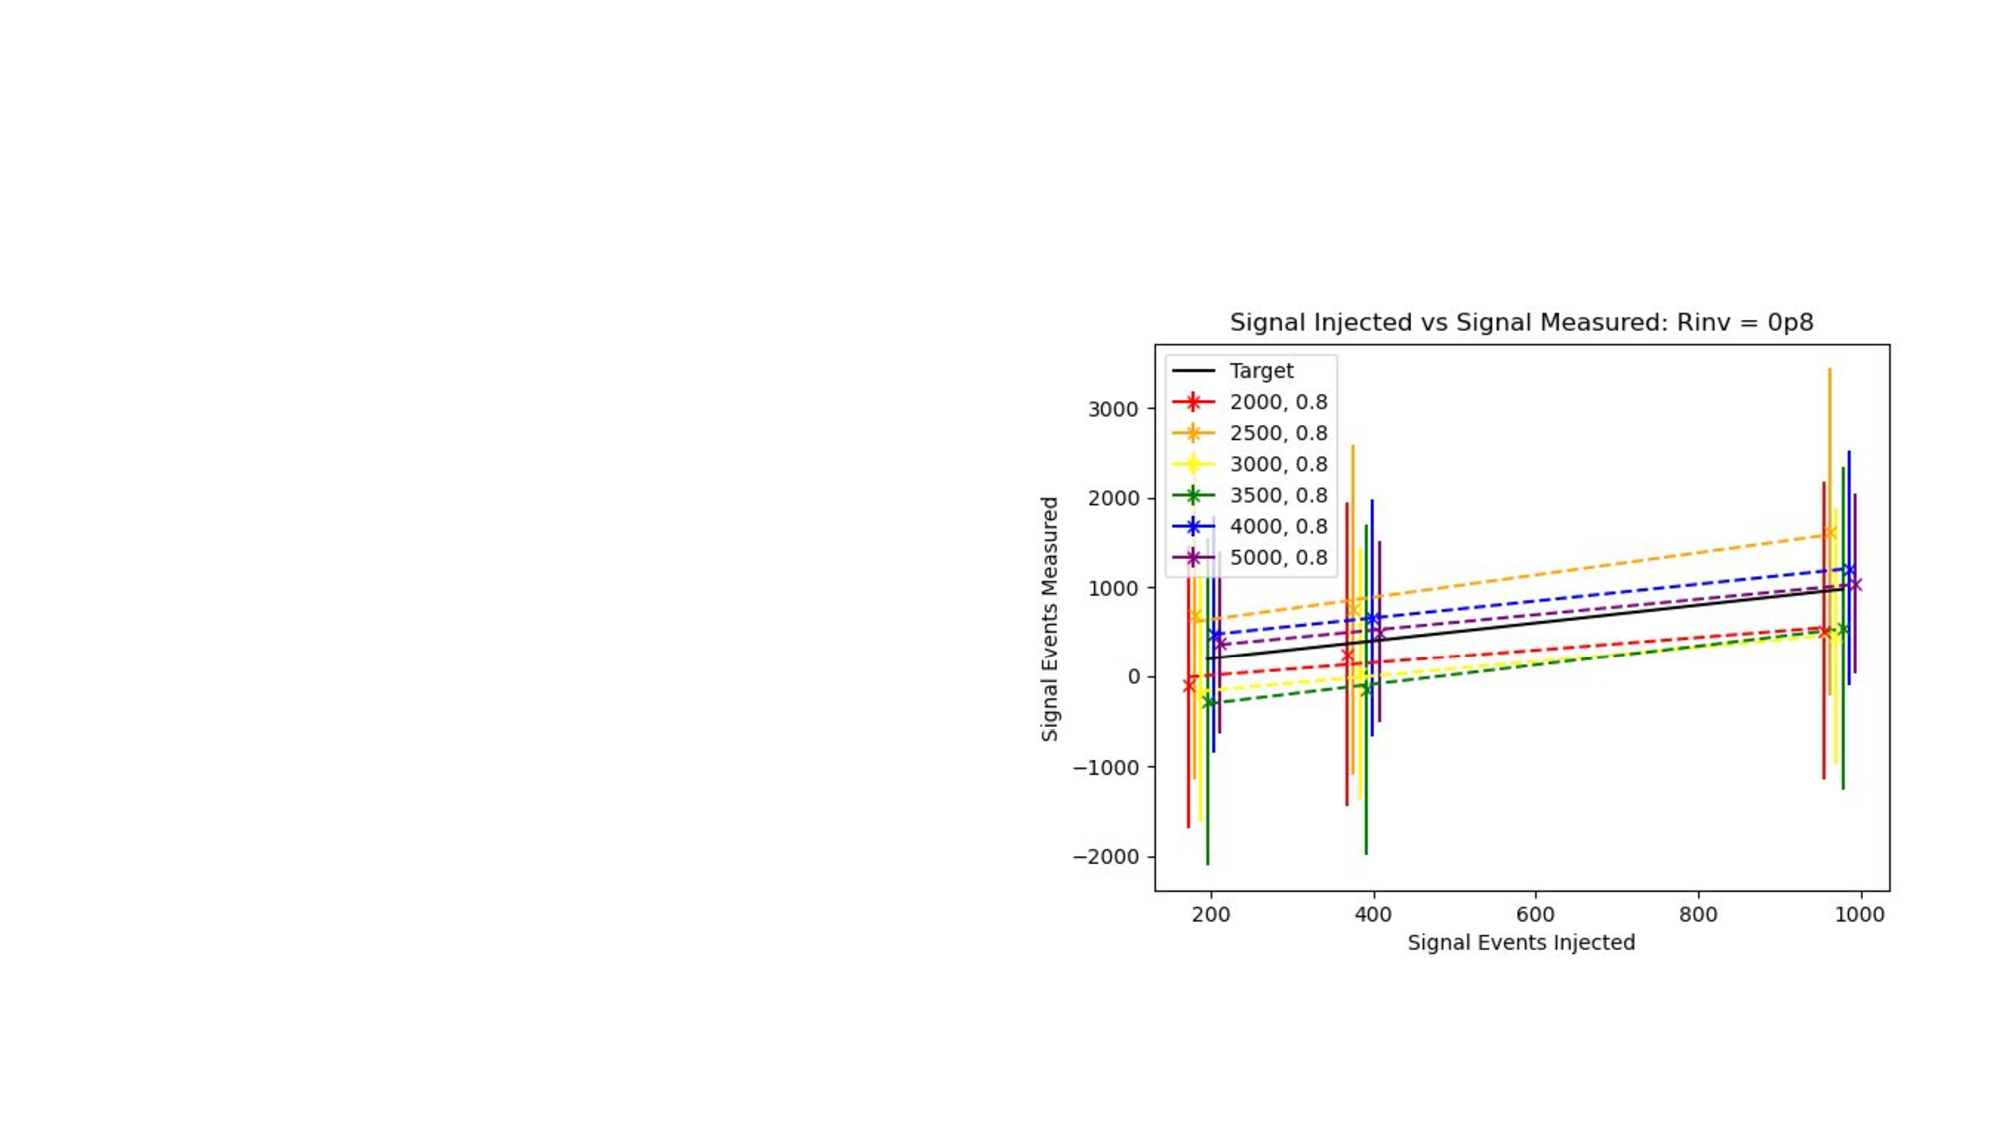
\includegraphics[width=0.45\textwidth]{figures/stats/siginj_asimov_08}
   \caption{Spurious signal at a variety of injected values (1, 2, and 5$\sigma$ significant), for all signal points in the grid, \rinv=0.2 (top left), 0.4 (top right), 0.6 (bottom left), and 0.8 (bottom right).
i%he requirement relative to $\sigma_{\text{fit}}$ is met for every signal point and injected signal size, thus satisfying the OR criteria from Equation~\ref{eq:spursig}.
    \label{fig:siginj_asimov}}
\end{figure}
\begin{figure}[!htbp]
\centering
   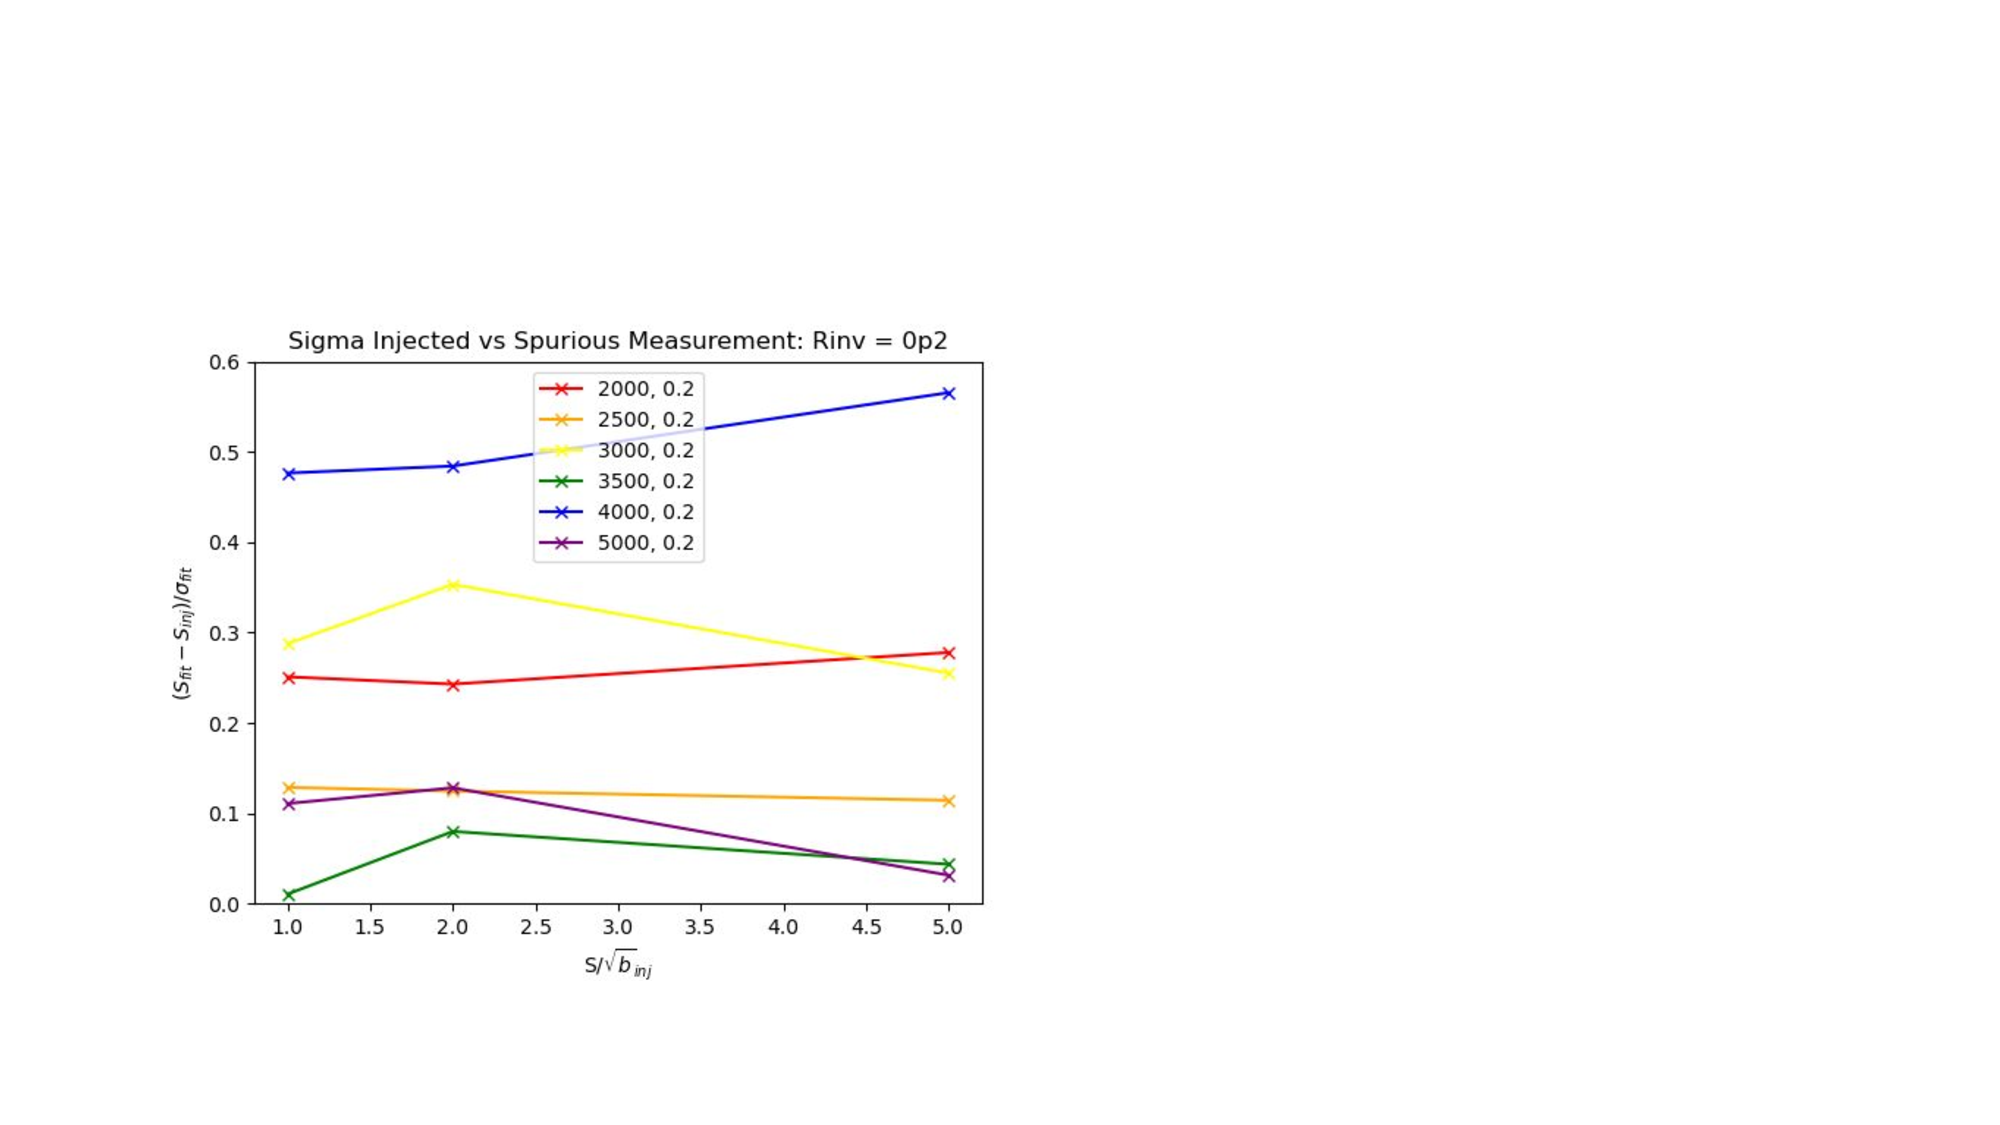
\includegraphics[width=0.45\textwidth]{figures/stats/siginj_asimov_02_check}
   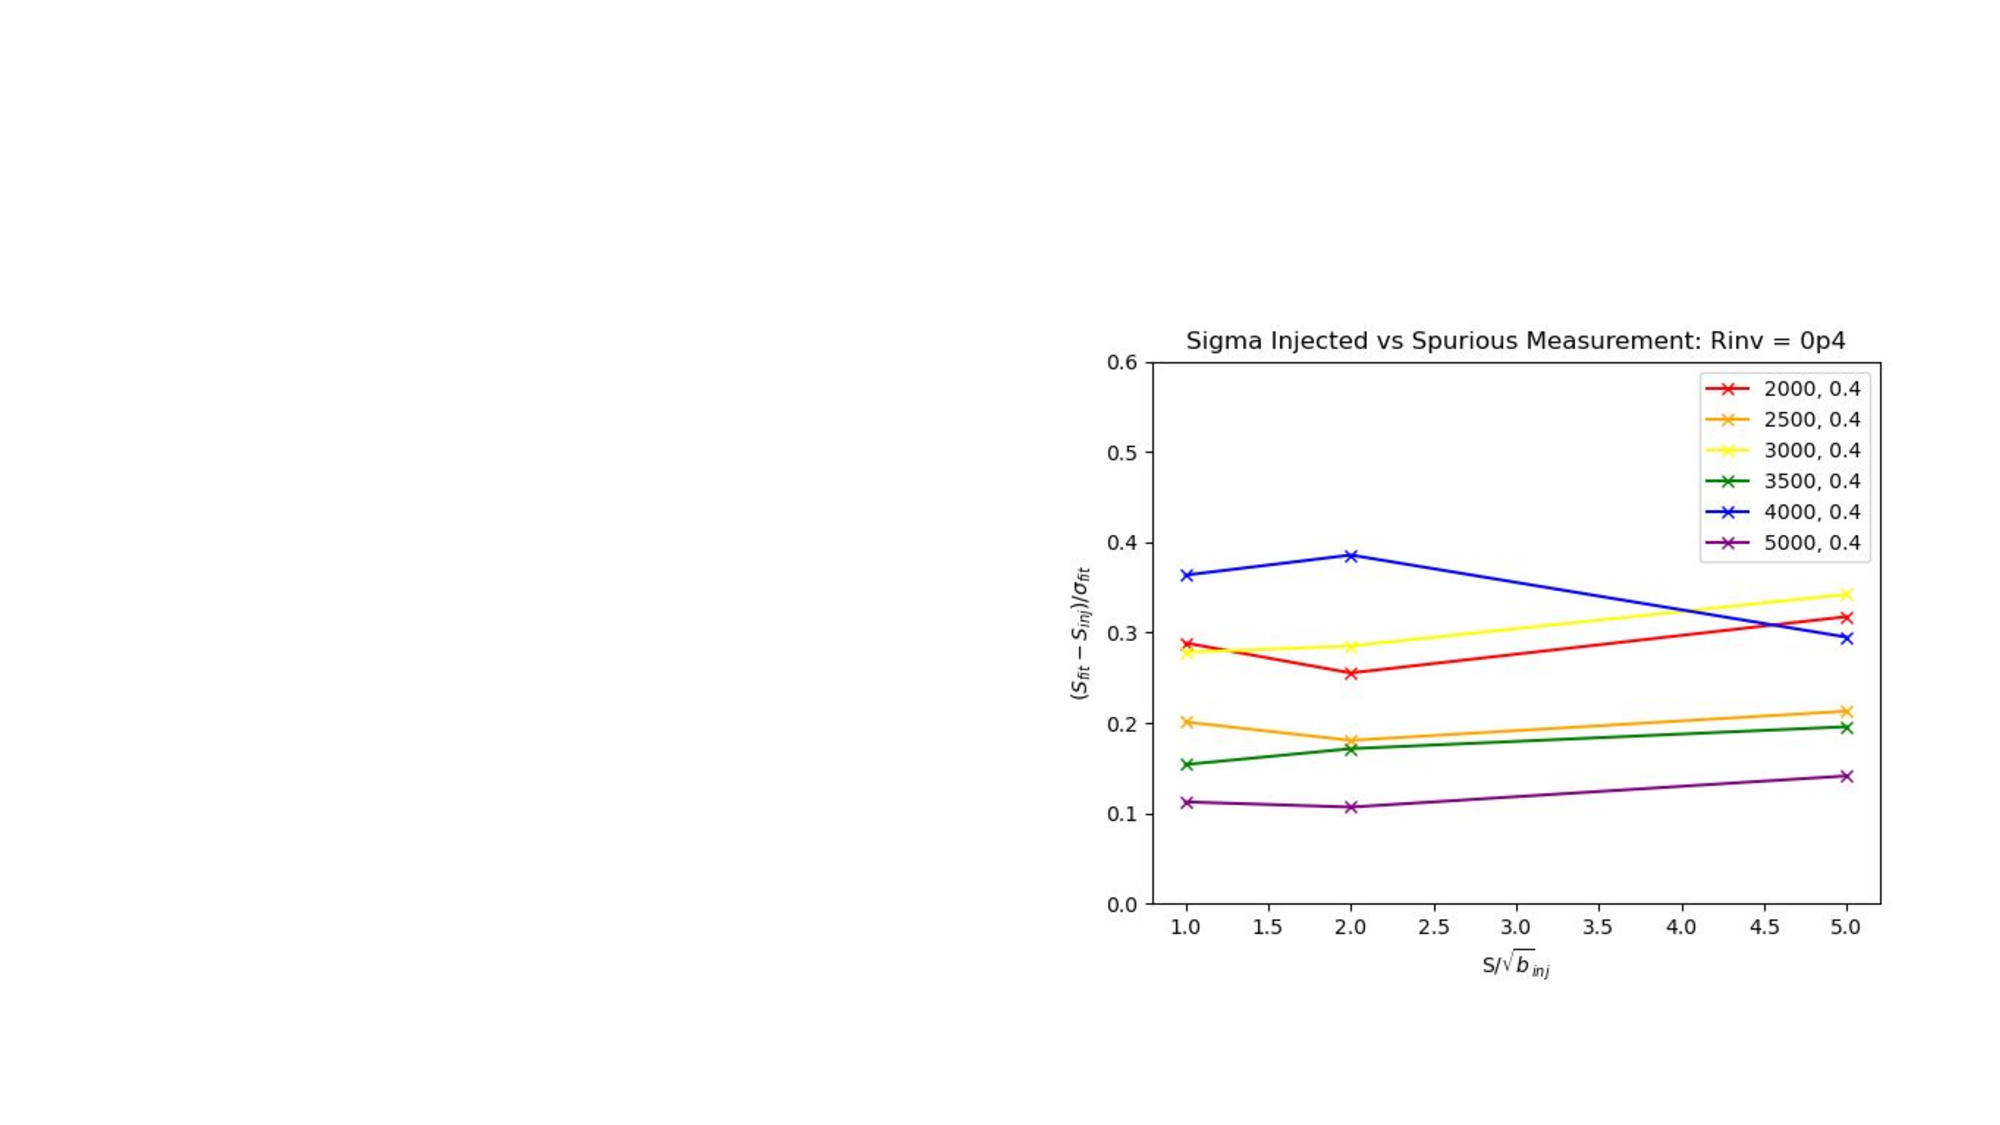
\includegraphics[width=0.45\textwidth]{figures/stats/siginj_asimov_04_check}
   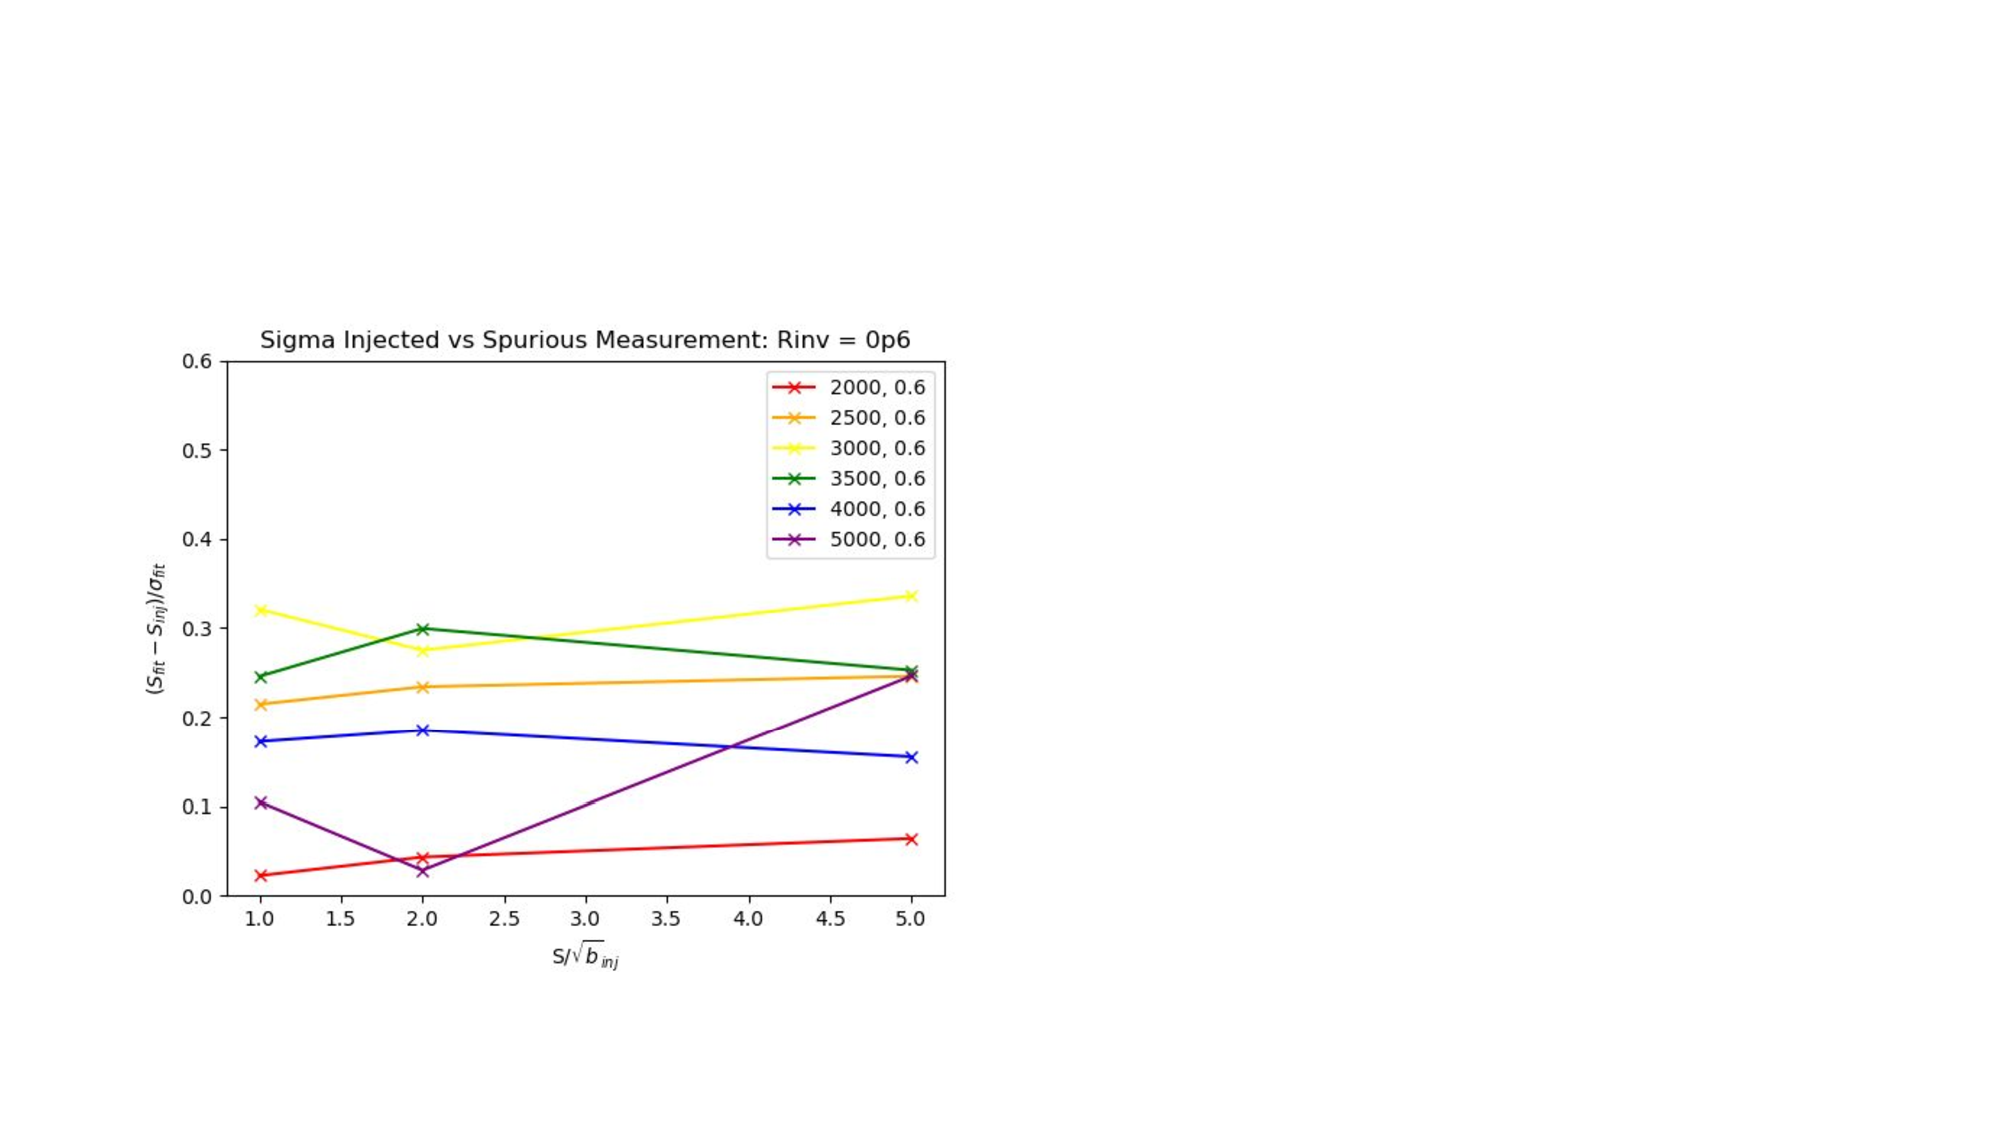
\includegraphics[width=0.45\textwidth]{figures/stats/siginj_asimov_06_check}
   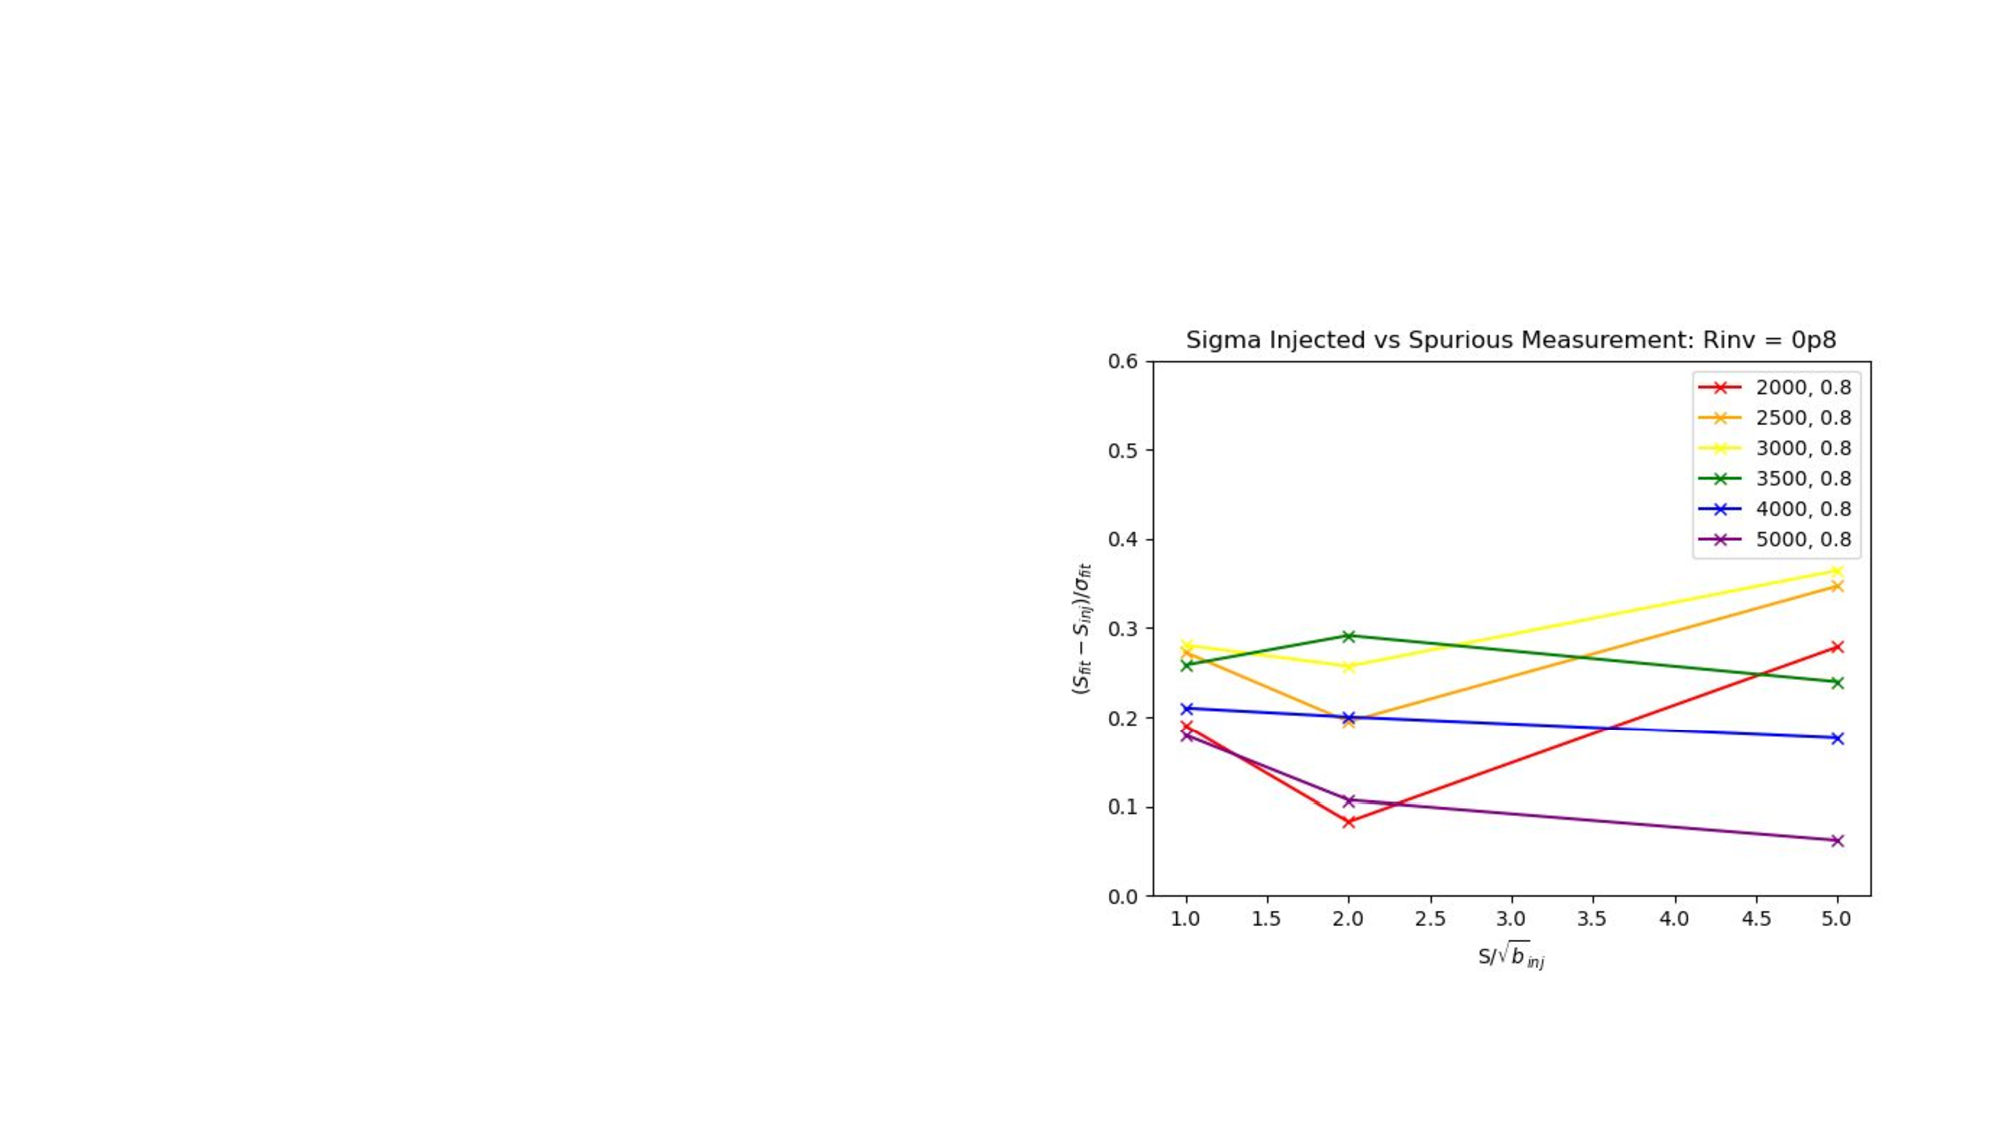
\includegraphics[width=0.45\textwidth]{figures/stats/siginj_asimov_08_check}
   \caption{S$_{\text{spur}}$/$\sigma_\text{fit}$ at a variety of injected values (1, 2, and 5$\sigma$ significant), for all signal points in the grid, \rinv=0.2 (top left), 0.4 (top right), 0.6 (bottom left), and 0.8 (bottom right).
i%he requirement relative to $\sigma_{\text{fit}}$ is met for every signal point and injected signal size, thus satisfying the OR criteria from Equation~\ref{eq:spursig}.
    \label{fig:siginj_asimov_check}}
\end{figure}


\clearpage

%------------------------------------------------- 
\subsubsection{Expected Sensitivity}
\label{subsec:fit_expsens}

Limits are obtained by determining the cross section of the signal that can be excluded to 95\% confidence. 
Figure~\ref{fig:limits_exp_1D} shows the expected limits obtained from S+B fits to statistically identical \mt~spectra from the CR region (which is closest in \mt~shape to the SR according to MC studies). 
%Figure~\ref{fig:limits_exp_1D_asimov} shows the expected limits obtained from an average of 50 Asimov toys thrown from the CR.
%The limits are very stable across individual data fits and Asimov, as well as across the CR and VR.
%The alignment of fluctuations between the single CR fit and Asimov toys indicates that the particular shape of data in the CR influences the shape of the limits.
%The limits shown come from an average of 10 Asimov pseudodata fits of the CR. Figure~\ref{fig:perc_success_limit} shows the percentage of Asimov limit tests that result in a successful fit. 

Considerable exclusion power is predicted for low \rinv~signal points, with the higher \rinv~points presenting more difficulty due to the very broad signal bump. 
A similar trend is observed in the CMS s-channel search~\cite{cms_schan}.

\begin{figure}[!htbp]
\centering
   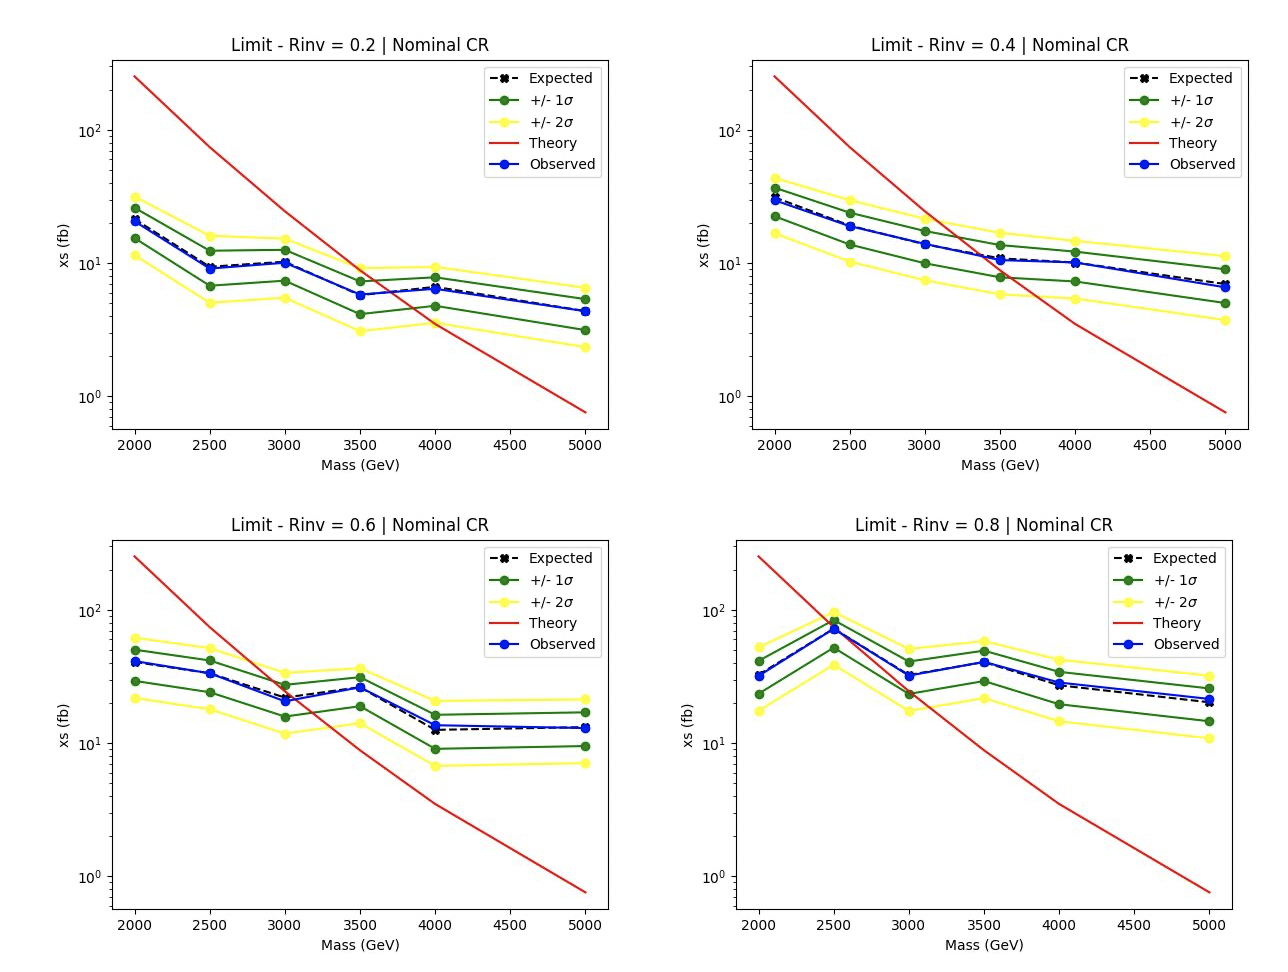
\includegraphics[width=0.95\textwidth]{figures/stats/limits_exp_1D}
    \caption{95\% C.L. upper limits for signal models across Z' mass, for four different \rinv~fractions, from the CR region (without systematics).
    \label{fig:limits_exp_1D}}
\end{figure}
%\begin{figure}[!htbp]
%\centering
%   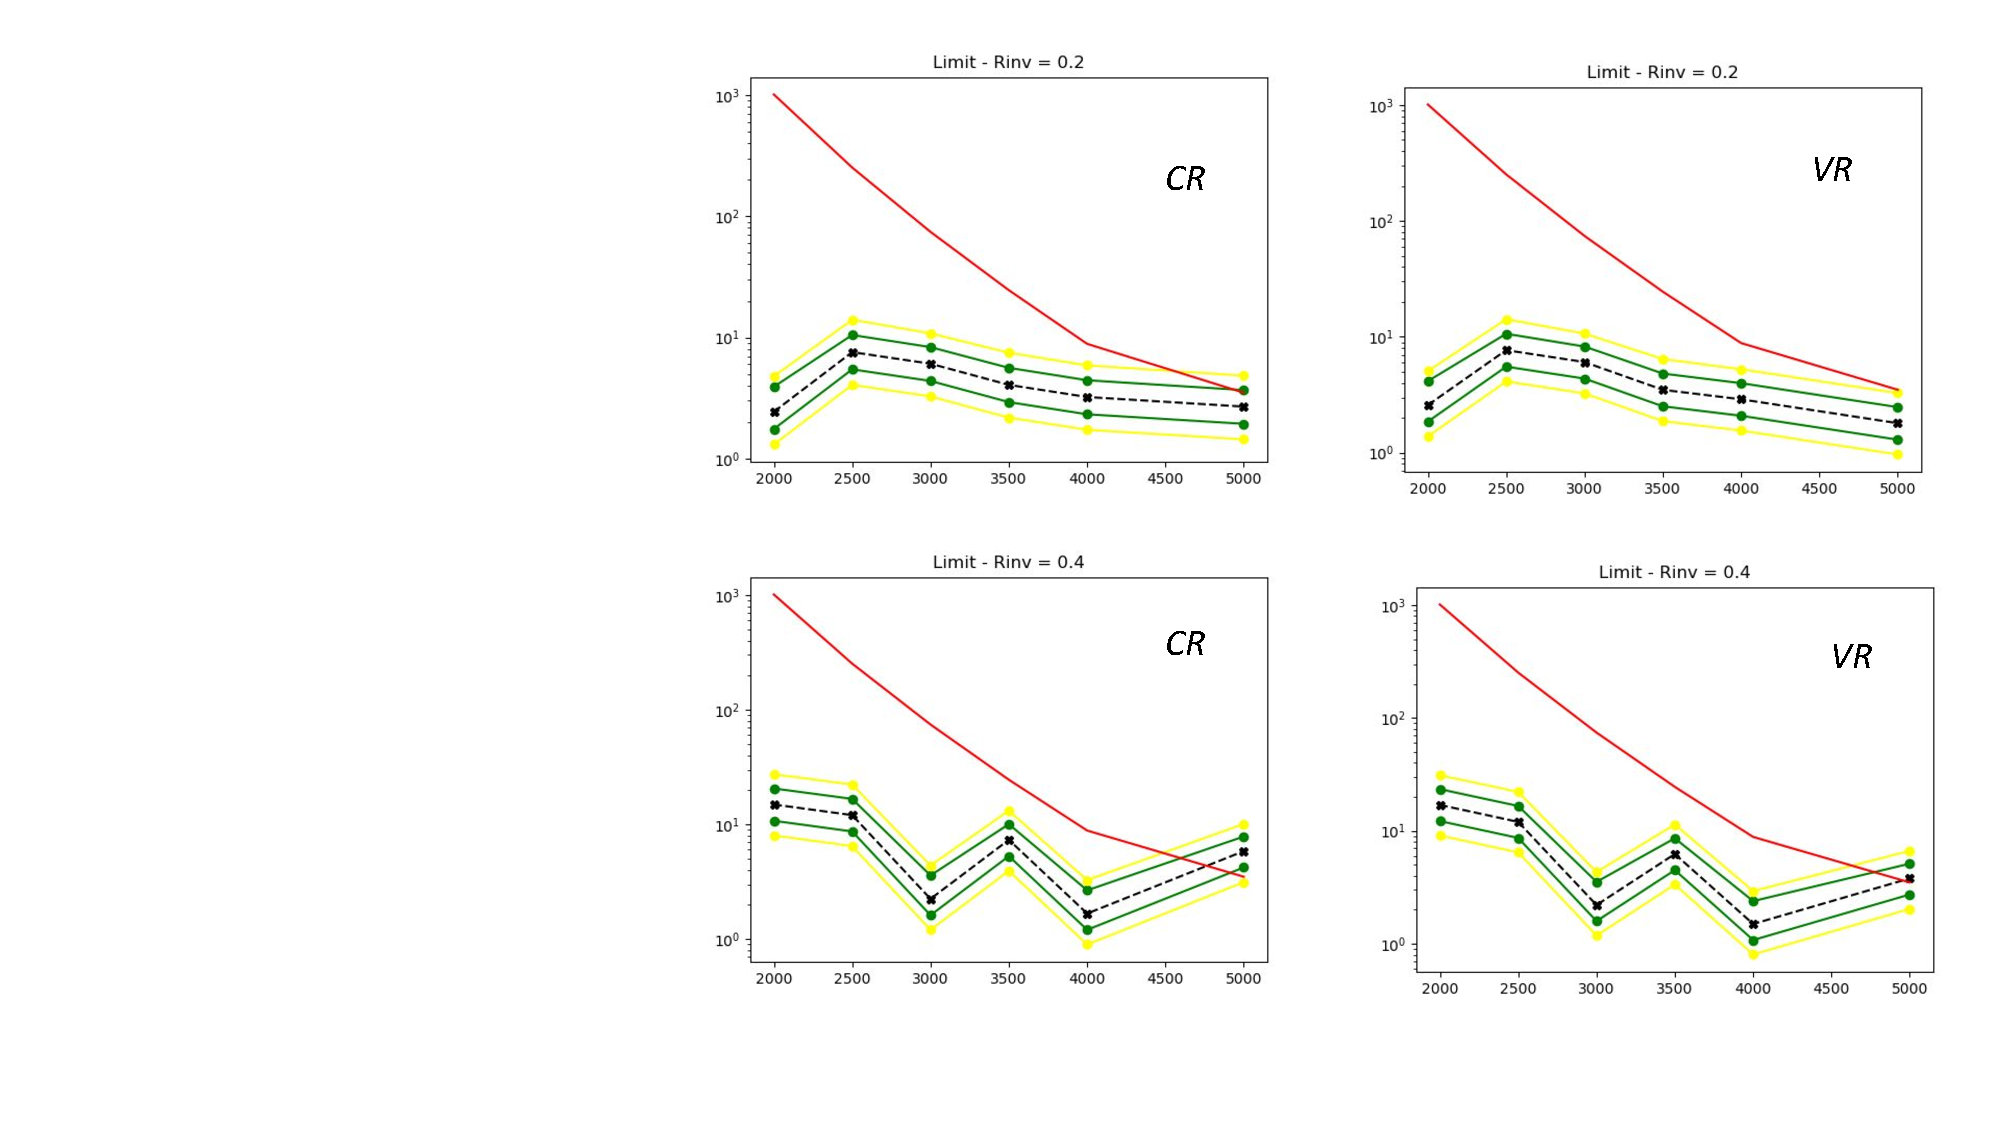
\includegraphics[width=0.9\textwidth]{figures/stats/limits_exp_1D_asimov_1}
%   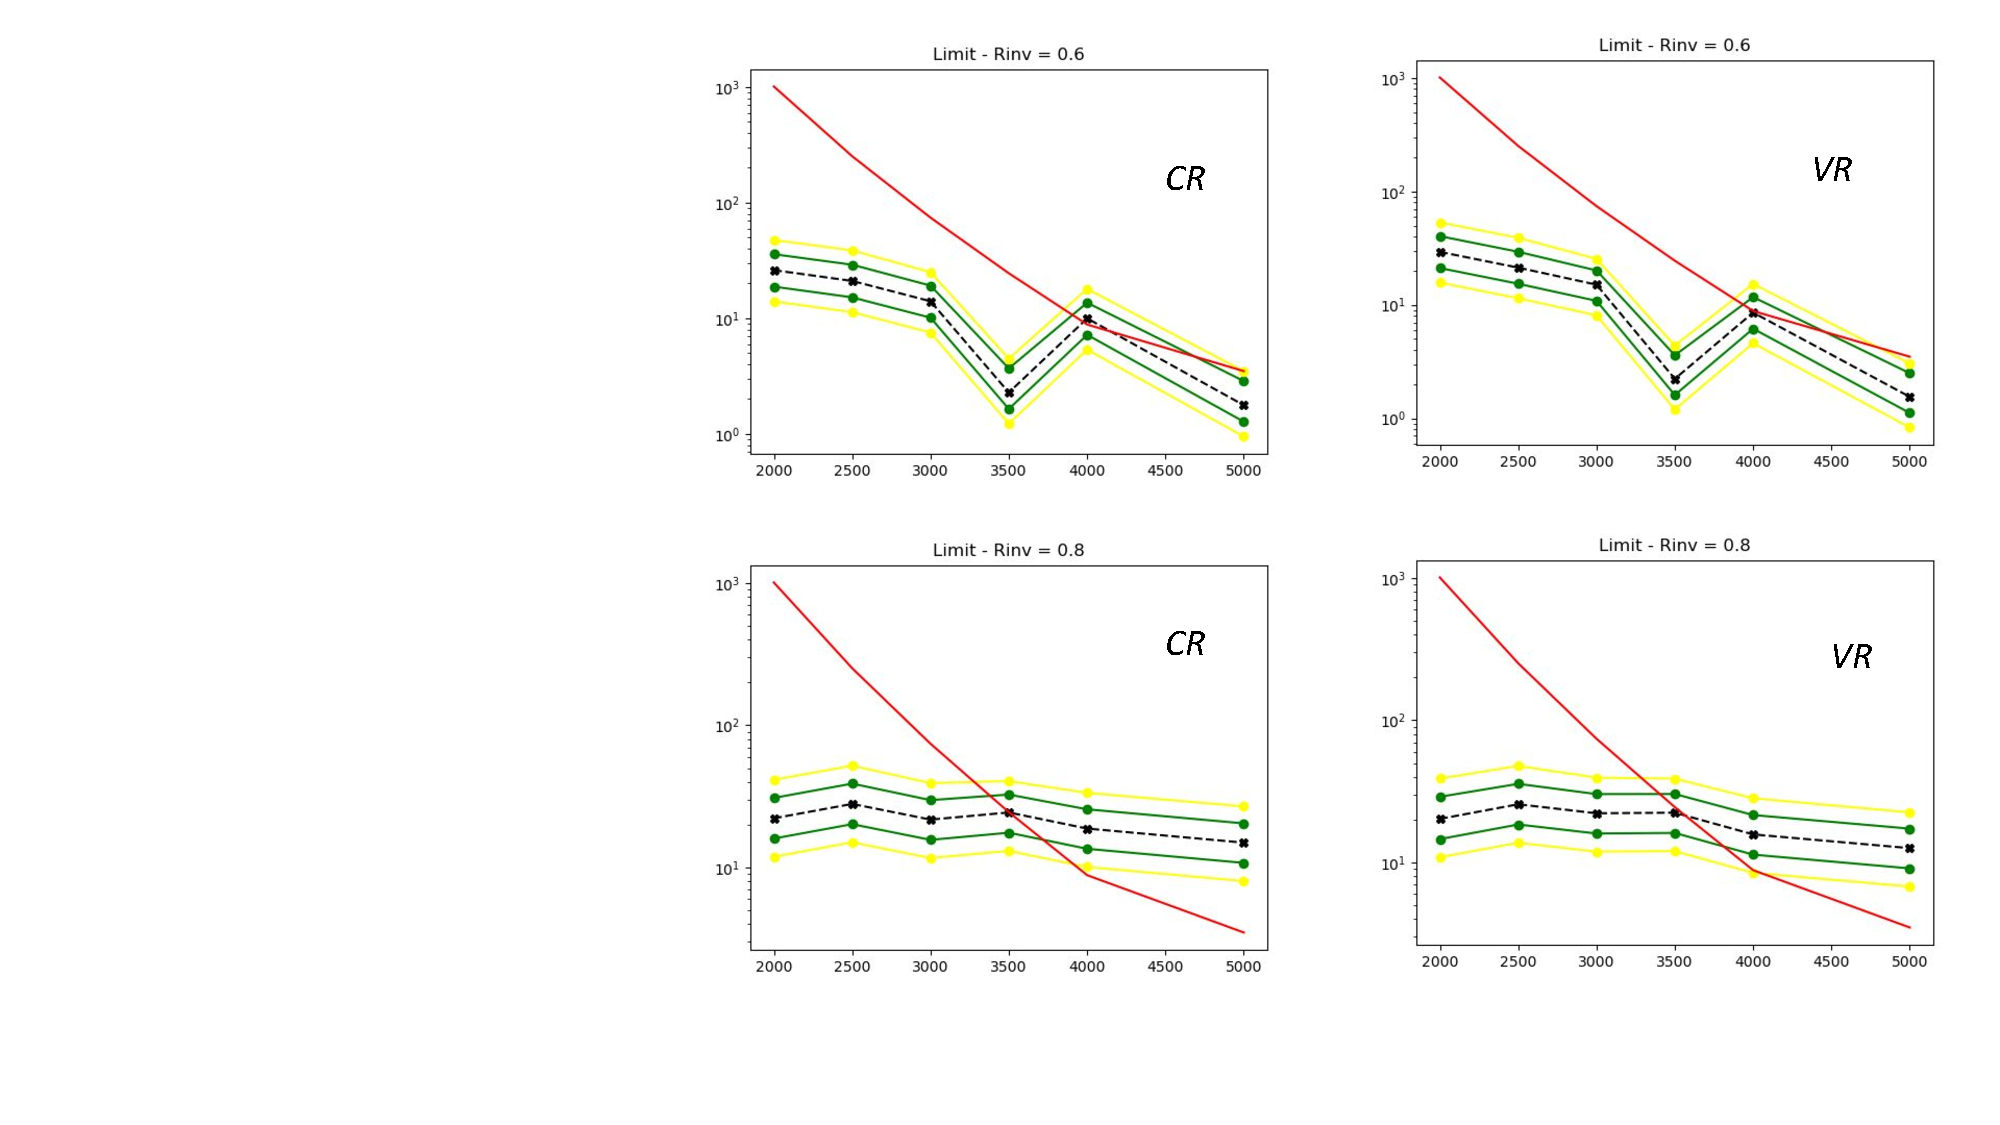
\includegraphics[width=0.9\textwidth]{figures/stats/limits_exp_1D_asimov_2}
%    \caption{95\% C.L. upper limits for signal models across Z' mass, for four different \rinv~fractions, using an average of 50 Asimov pseudo-data tests from the CR (left) and VR (right) (without systematics).
%    \label{fig:limits_exp_1D_asimov}}
%\end{figure}

%\begin{figure}[!htbp]
%\centering
%   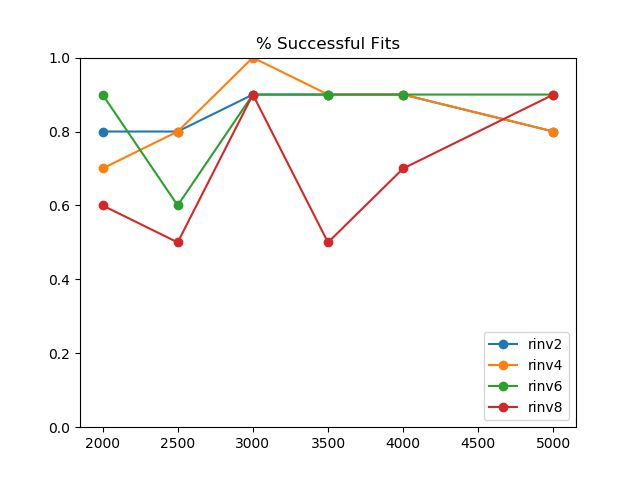
\includegraphics[width=0.6\textwidth]{figures/stats/perc_success_limit}
%    \caption{Percent of Asimov pseudodata S+B fits with successful fit and successful limit convergence.
%    \label{fig:perc_success_limit}}
%\end{figure}

A 2D limit presentation is also being considered, in the (\rinv, mass) plane.


\clearpage


